% !TeX root = ../thesis.tex
\chapter{KẾT QUẢ THỰC HIỆN}

% !TeX root = ../thesis.tex

%

\section{Giới thiệu}
Chương này trình bày kết quả mô phỏng hệ thống robot bốn chân sử dụng nền tảng ROS~2 Humble \cite{ros2docs} kết hợp với trình mô phỏng Gazebo Classic \cite{gazebo}. Trước khi triển khai trên mô phỏng phức tạp Gazebo, bộ điều khiển PID được mô hình hóa và kiểm chứng sơ bộ trên môi trường Matlab/Simulink để xác minh tính đáp ứng động học. Mục tiêu của toàn bộ quá trình mô phỏng là xác minh tính đúng đắn của các thuật toán lập kế hoạch quỹ đạo, động học nghịch (Inverse Kinematics), và bộ điều khiển PID trước khi triển khai trên robot thực. Toàn bộ kết quả được trình bày thông qua các hình minh họa, bao gồm cấu hình mô phỏng, trực quan hóa quá trình hoạt động, đánh giá quỹ đạo bàn chân, biên dạng góc khớp và hiệu năng bộ điều khiển PID.

Nội dung chương được tổ chức như sau: Mục~5.2 trình bày mô phỏng và đánh giá bộ điều khiển bằng Matlab/Simulink; Mục~5.3 trình bày cấu hình chi tiết của môi trường mô phỏng Gazebo; Mục~5.4 đánh giá hiệu năng bộ điều khiển PID nâng cao cùng với quỹ đạo sinh ra trên mô phỏng; và Mục~5.5 trình bày kết quả thực nghiệm trên phần cứng cùng phân tích so sánh sim-to-real.

\section{Mô phỏng và đánh giá bộ điều khiển bằng Matlab/Simulink}

Để kiểm chứng bộ điều khiển PID trước khi đưa vào hệ thống thực tế hoặc môi trường mô phỏng Gazebo, toàn bộ hệ thống động học và điều khiển của robot được mô hình hóa trên môi trường Matlab/Simulink. Hệ thống được tổ chức thành một vòng lặp kín (Closed-loop) hoàn chỉnh như thể hiện trong Hình~\ref{fig:simulink_block_diagram}. Chu trình điều khiển bao gồm 3 khối chức năng chính: khối đối tượng vật lý (Quadruped Robot) cung cấp phản hồi trạng thái, khối điều khiển (PID Controller) tính toán tín hiệu bù, và khối thực thi (Execution) chuyển đổi lệnh bù thành góc khớp.

\begin{figure}[H]
    \centering
    
\includegraphics[width=\textwidth]{img_matlab/fig1-PID-controller.png}
    \caption{Sơ đồ khối tổng thể vòng lặp kín điều khiển tư thế robot}
    \label{fig:simulink_block_diagram}
\end{figure}

\subsection{Mô hình toán học đối tượng (Quadruped Robot)}
Khối Quadruped Robot (Hình~\ref{fig:simulink_quadruped_robot}) đóng vai trò là "môi trường vật lý ảo" của hệ thống. Đầu vào của khối này là bộ $12$ lệnh góc khớp $\theta$ sinh ra từ bộ điều khiển. Đầu ra là các giá trị cao độ bàn chân (\texttt{z\_out}) và phản hồi cảm biến IMU (\texttt{roll\_meas}, \texttt{pitch\_meas}). Sơ đồ này mô phỏng quy trình thu thập trạng thái cơ cấu chấp hành để tái tạo lại tư thế định hướng của thân robot.

\begin{figure}[H]
    \centering
    
\includegraphics[width=0.8\textwidth]{img_matlab/fig3-quadruped-robot.png}
    \caption{Cấu trúc khối đối tượng mô phỏng phản hồi trạng thái (Quadruped Robot)}
    \label{fig:simulink_quadruped_robot}
\end{figure}

Sâu bên trong khối Robot, Hình~\ref{fig:simulink_forward_kinematics} phơi bày cấu trúc mô hình hóa động học của robot. Tại đây, hệ thống sử dụng 4 khối \texttt{Universal\_FK} chạy song song để giải phương trình động học thuận cho 4 chân. Từ các góc khớp $\theta_{1,2,3}$ của từng chân, mô hình ánh xạ ra tọa độ không gian thực $(x, y, z)$ của bàn chân đối với hệ quy chiếu thân robot. Giá trị \texttt{z\_out} thu được chính là cơ sở toán học để mô phỏng trạng thái nghiêng thân và xác định độ cân bằng của toàn hệ thống trong không gian 3D.

\begin{figure}[H]
    \centering
    
\includegraphics[width=\textwidth]{img_matlab/fig4-mo-hinh-hoa-robot.png}
    \caption{Cấu trúc mô hình hóa động học robot (dựa trên phương trình Động học thuận)}
    \label{fig:simulink_forward_kinematics}
\end{figure}

\subsection{Thiết kế bộ điều khiển PID và tiền xử lý tín hiệu}
Tín hiệu phản hồi từ mô hình Robot tiếp tục được đưa vào khối PID Controller (Hình~\ref{fig:pid_simulink_detail}). Khối này không chỉ thực hiện tính toán P-I-D đơn thuần mà còn bao hàm toàn bộ chuỗi tiền xử lý tín hiệu (Signal Processing Pipeline) để giải quyết hiện tượng nhiễu động học. Tín hiệu thô từ IMU trải qua 3 cấp độ lọc: lọc trung bình trượt hàm mũ (EMA), lọc thông thấp (Avg) để trích xuất sai lệch đường cơ sở, và cuối cùng là đi qua vùng chết (Deadzone). Chỉ những sai lệch đã qua thanh lọc này mới được đưa vào bộ điều khiển Rời rạc \texttt{PID(z)} để xuất ra lệnh bù tư thế (\texttt{roll\_correction}, \texttt{pitch\_correction}), đảm bảo hệ thống phản ứng trơn tru mà không bị đánh lừa bởi dao động bước đi tự nhiên.

\begin{figure}[H]
    \centering
    
\includegraphics[width=0.8\textwidth]{img_matlab/fig5-PID.png}
    \caption{Chi tiết cấu trúc chuỗi tiền xử lý tín hiệu và khối điều khiển PID rời rạc}
    \label{fig:pid_simulink_detail}
\end{figure}

\subsection{Khối thực thi động học nghịch (Execution)}
Cuối cùng, vòng lặp điều khiển được khép kín tại khối Execution (Hình~\ref{fig:pid_execution_flow}). Nhiệm vụ của khối này là giải quyết bài toán Động học nghịch (Inverse Kinematics). Đầu vào là tín hiệu bù góc Roll và Pitch; đầu ra là tập hợp $12$ quỹ đạo góc khớp \texttt{th1}, \texttt{th2}, \texttt{th3} của 4 chân. Sơ đồ minh họa quá trình ánh xạ ngược: từ yêu cầu duy trì mặt phẳng thăng bằng cho thân robot, khối Execution phân bổ độ dịch chuyển theo trục Z (\texttt{z\_foot\_ref}) xuống từng cơ cấu chân, buộc các động cơ phải tự động gập/duỗi để đáp ứng bù trừ sai lệch theo thời gian thực.

\begin{figure}[H]
    \centering
    
\includegraphics[width=0.8\textwidth]{img_matlab/fig2-execution.png}
    \caption{Cấu trúc khối thực thi giải tích động học nghịch (Inverse Kinematics) cho 4 chân}
    \label{fig:pid_execution_flow}
\end{figure}

\subsection{Kết quả mô phỏng}

\subsubsection*{Quá trình hiệu chỉnh (Tuning) bộ điều khiển PID độc lập cho trục Roll và Pitch}
Trong thực tế, đặc tính động học của robot trên hai trục Roll và Pitch không hoàn toàn giống nhau do sự phân bố khối lượng và khoảng cách các chân (chiều dài cơ sở và chiều rộng cơ sở) khác biệt. Do đó, bộ điều khiển PID được thiết kế để hiệu chỉnh (tuning) độc lập cho từng trục. Quá trình hiệu chỉnh được thực hiện tuần tự từ khâu tỷ lệ (P), vi phân (D) đến tích phân (I) nhằm đạt được sự cân bằng tối ưu giữa tốc độ đáp ứng và độ ổn định.

\textbf{\textit{Hiệu chỉnh bộ điều khiển trục Roll}}

Đầu tiên, khâu tỷ lệ được áp dụng với hệ số $K_p=4$ (Hình~\ref{fig:roll_tuning_p}). Hệ thống đáp ứng nhanh với nhiễu bước $0{,}15$ rad tại $t=3$ s, góc nghiêng giảm mạnh nhưng xảy ra hiện tượng dao động lớn, kéo dài liên tục và tồn tại sai số xác lập rõ rệt quanh mức $0{,}025$ rad.
Tiếp theo, thành phần vi phân được thêm vào ($K_p=4, K_d=1{,}3$) (Hình~\ref{fig:roll_tuning_pd}). Nhờ khả năng dự báo sự thay đổi của khâu D, các dao động được dập tắt nhanh chóng sau khoảng $10$ s, hệ thống trở nên trơn tru hơn nhưng sai số xác lập vẫn chưa được loại bỏ.
Cuối cùng, khâu tích phân được đưa vào ($K_p=4, K_i=1{,}2, K_d=1{,}3$) (Hình~\ref{fig:roll_tuning_pid}). Tại thời điểm này, sai số xác lập bị triệt tiêu hoàn toàn, góc đo được (\texttt{roll\_meas}) từ từ hội tụ chính xác về điểm đặt (setpoint) $0$ rad.

\begin{figure}[H]
    \centering
    \begin{subfigure}[b]{0.48\textwidth}
        \centering
        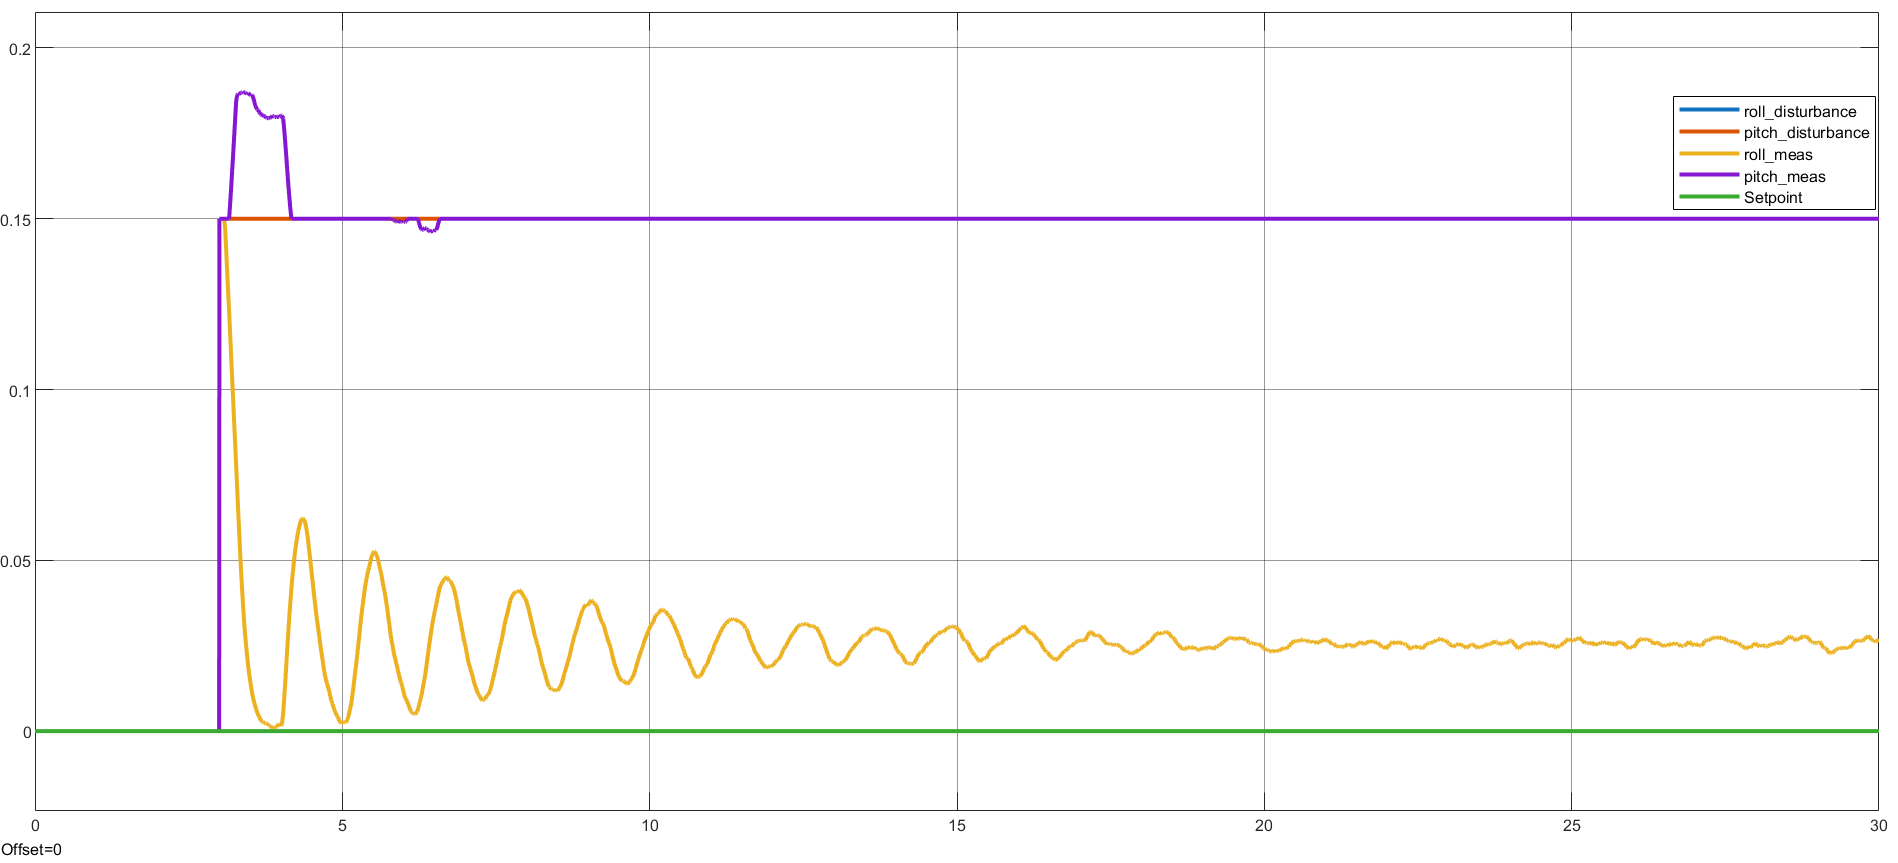
\includegraphics[width=\textwidth]{Images/PID_turning/PID_turning/roll turning Kp=4.png}
        \caption{Chỉ dùng khâu P ($K_p=4$)}
        \label{fig:roll_tuning_p}
    \end{subfigure}
    \hfill
    \begin{subfigure}[b]{0.48\textwidth}
        \centering
        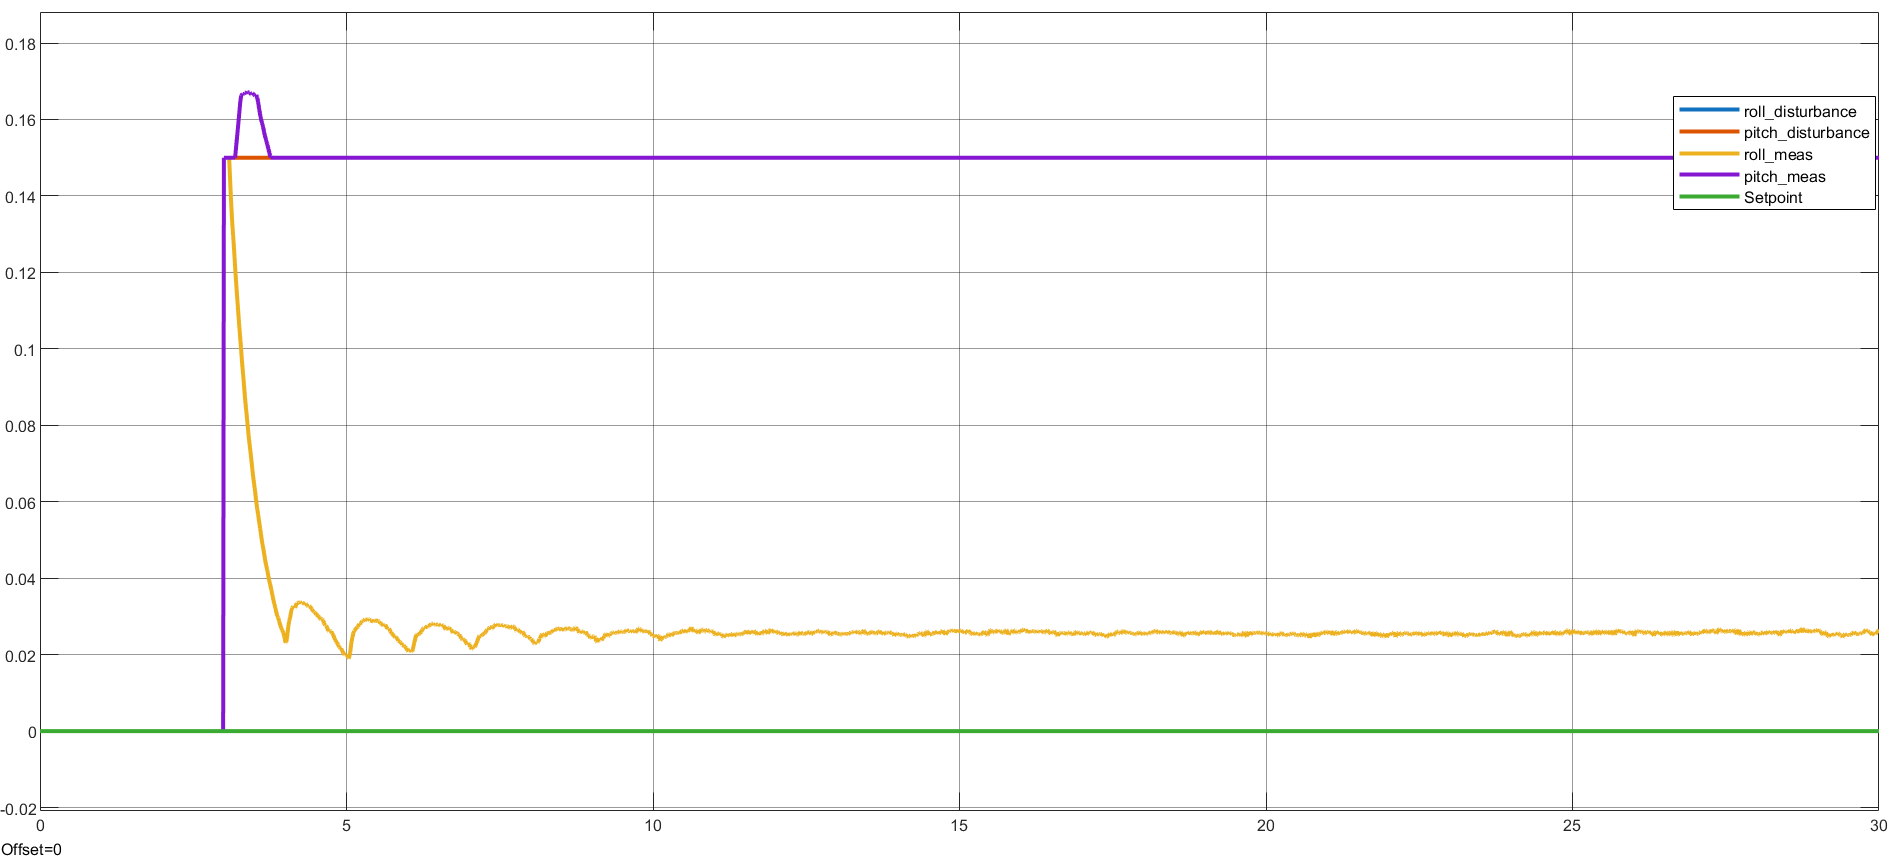
\includegraphics[width=\textwidth]{Images/PID_turning/PID_turning/roll turning Kp=4 Kd=1.3.png}
        \caption{Dùng khâu PD ($K_p=4, K_d=1{,}3$)}
        \label{fig:roll_tuning_pd}
    \end{subfigure}
    
    \vspace{0.2cm}
    \begin{subfigure}[b]{0.6\textwidth}
        \centering
        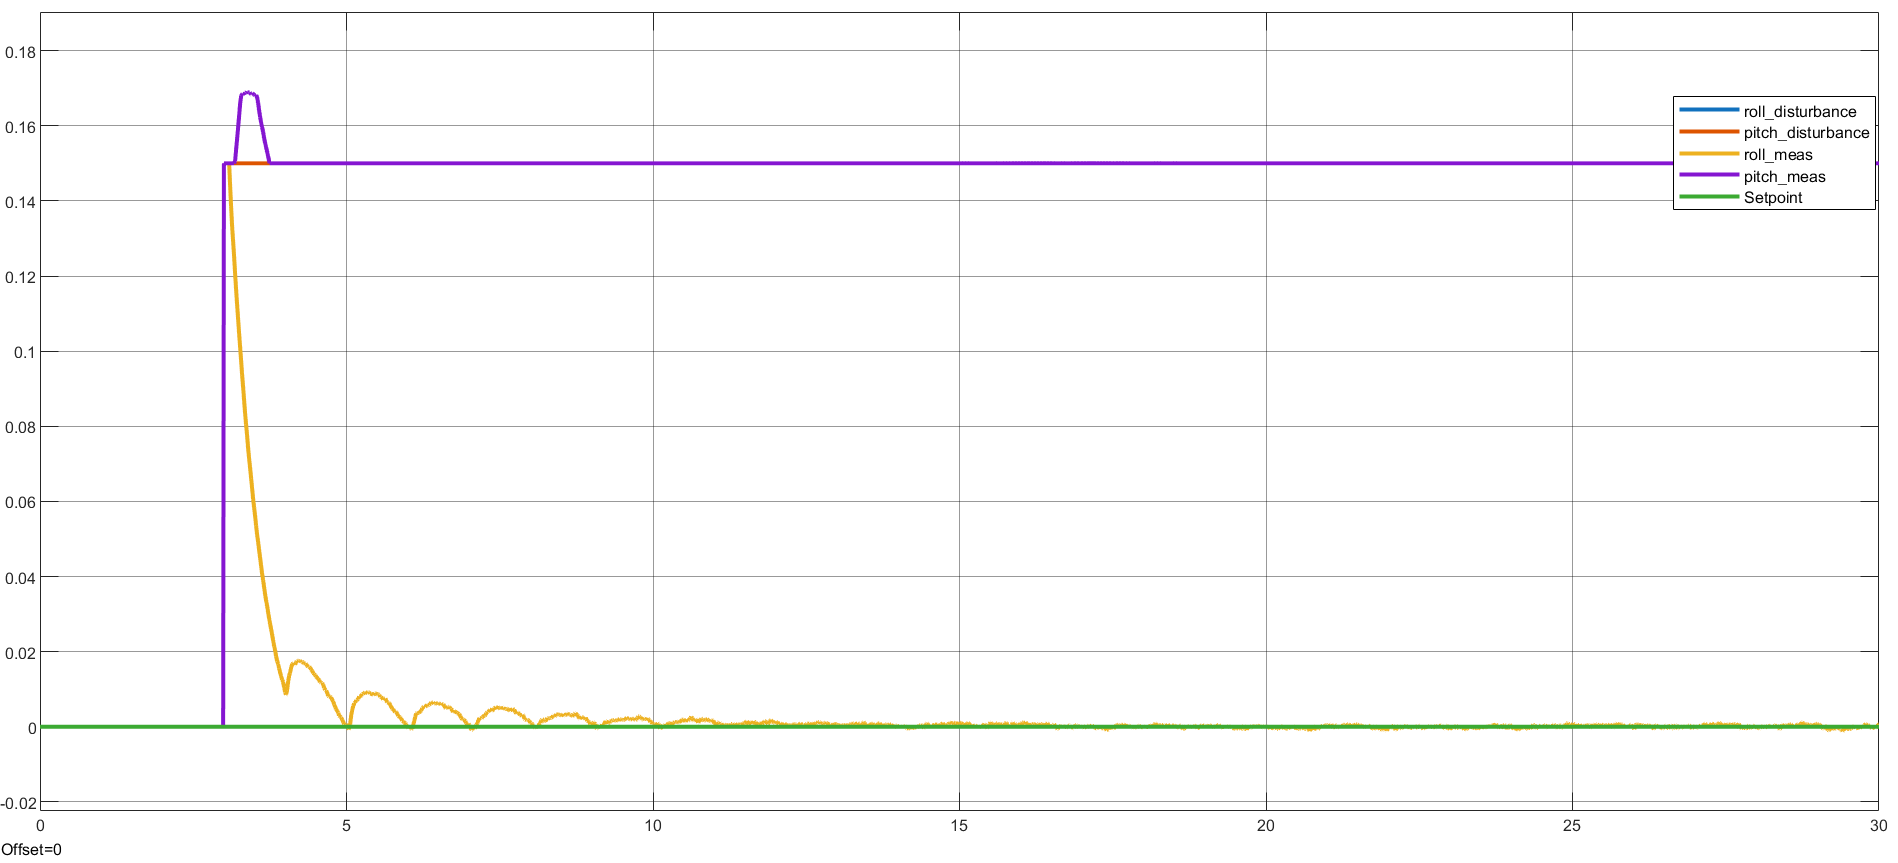
\includegraphics[width=\textwidth]{Images/PID_turning/PID_turning/roll turning Kp=4 Kd=1.3 Ki=1.2.png}
        \caption{Dùng PID hoàn chỉnh ($K_p=4, K_i=1{,}2, K_d=1{,}3$)}
        \label{fig:roll_tuning_pid}
    \end{subfigure}
    \caption{Quá trình hiệu chỉnh các khâu P, D, I cho trục Roll}
    \label{fig:roll_tuning_process}
\end{figure}

\textbf{\textit{Hiệu chỉnh bộ điều khiển trục Pitch}}

Quá trình tương tự được thực hiện cho trục Pitch. Trục này yêu cầu lực bù lớn hơn một chút để chống lại mô-men quán tính theo trục dọc của robot.
Với khâu P ($K_p=5$) (Hình~\ref{fig:pitch_tuning_p}), hệ thống giảm được sai lệch nhưng vẫn dao động. Khi thêm khâu D ($K_p=5, K_d=1{,}3$) (Hình~\ref{fig:pitch_tuning_pd}), dao động được dập tắt nhanh chóng. Cuối cùng, khâu I được bổ sung ($K_p=5, K_i=1{,}6, K_d=1{,}3$) (Hình~\ref{fig:pitch_tuning_pid}) giúp triệt tiêu hoàn toàn sai số xác lập, đưa hệ thống về điểm làm việc tối ưu $0$ rad.

\begin{figure}[H]
    \centering
    \begin{subfigure}[b]{0.48\textwidth}
        \centering
        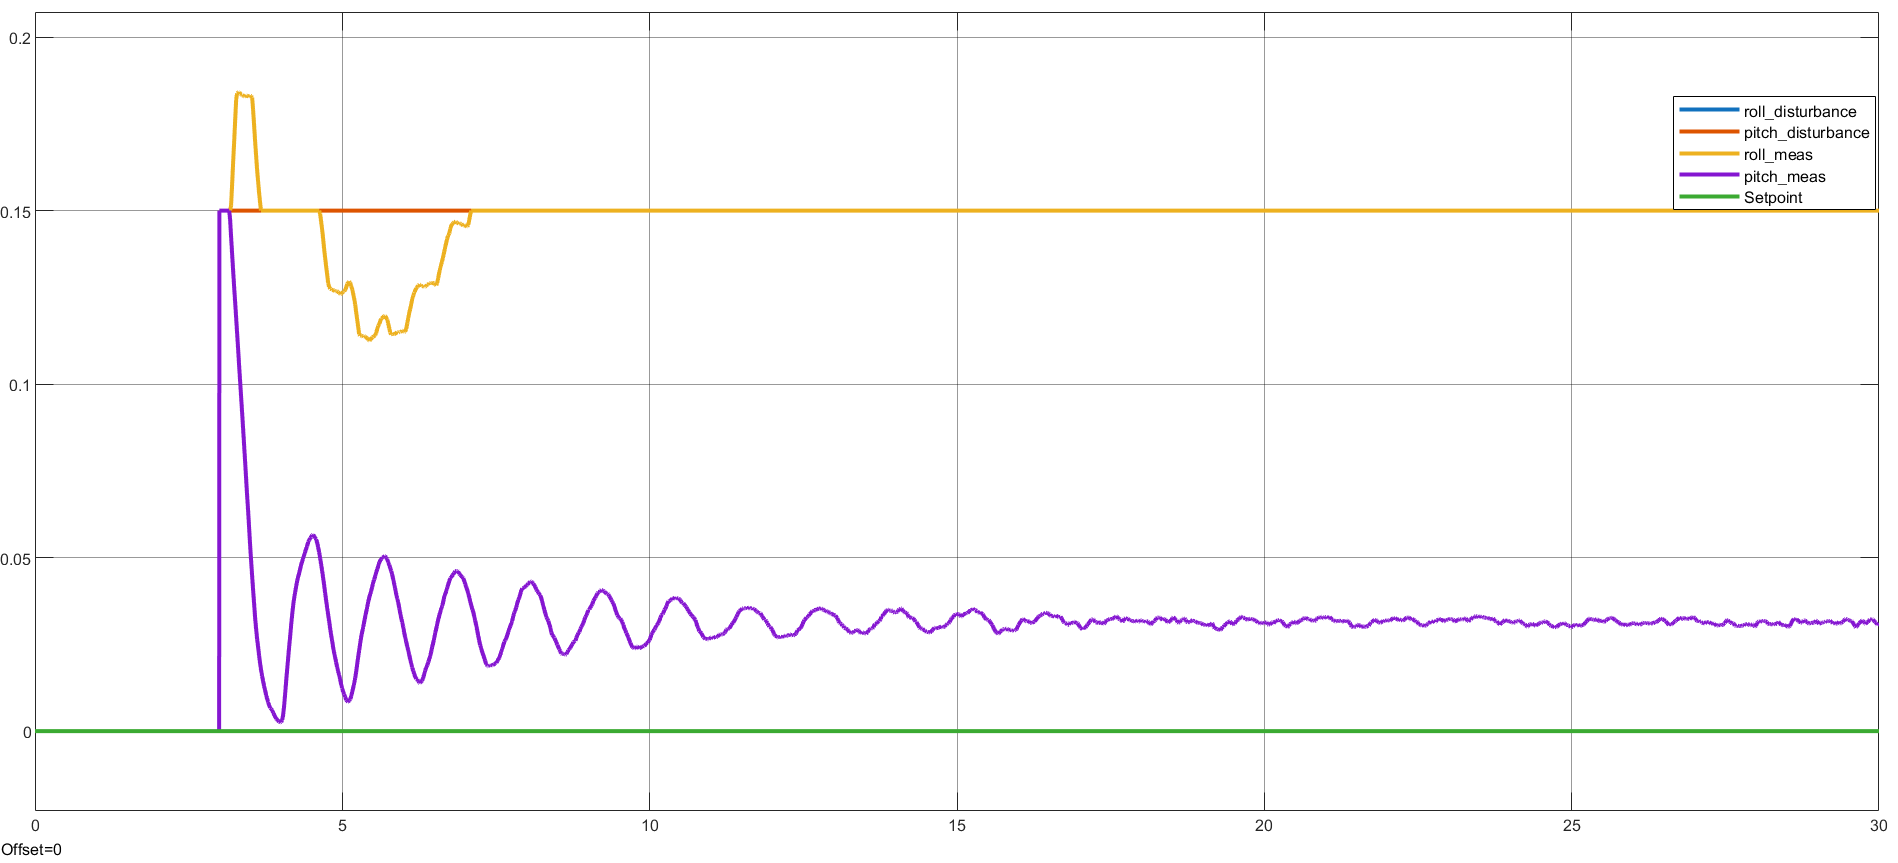
\includegraphics[width=\textwidth]{Images/PID_turning/PID_turning/pitch turning Kp=5.png}
        \caption{Chỉ dùng khâu P ($K_p=5$)}
        \label{fig:pitch_tuning_p}
    \end{subfigure}
    \hfill
    \begin{subfigure}[b]{0.48\textwidth}
        \centering
        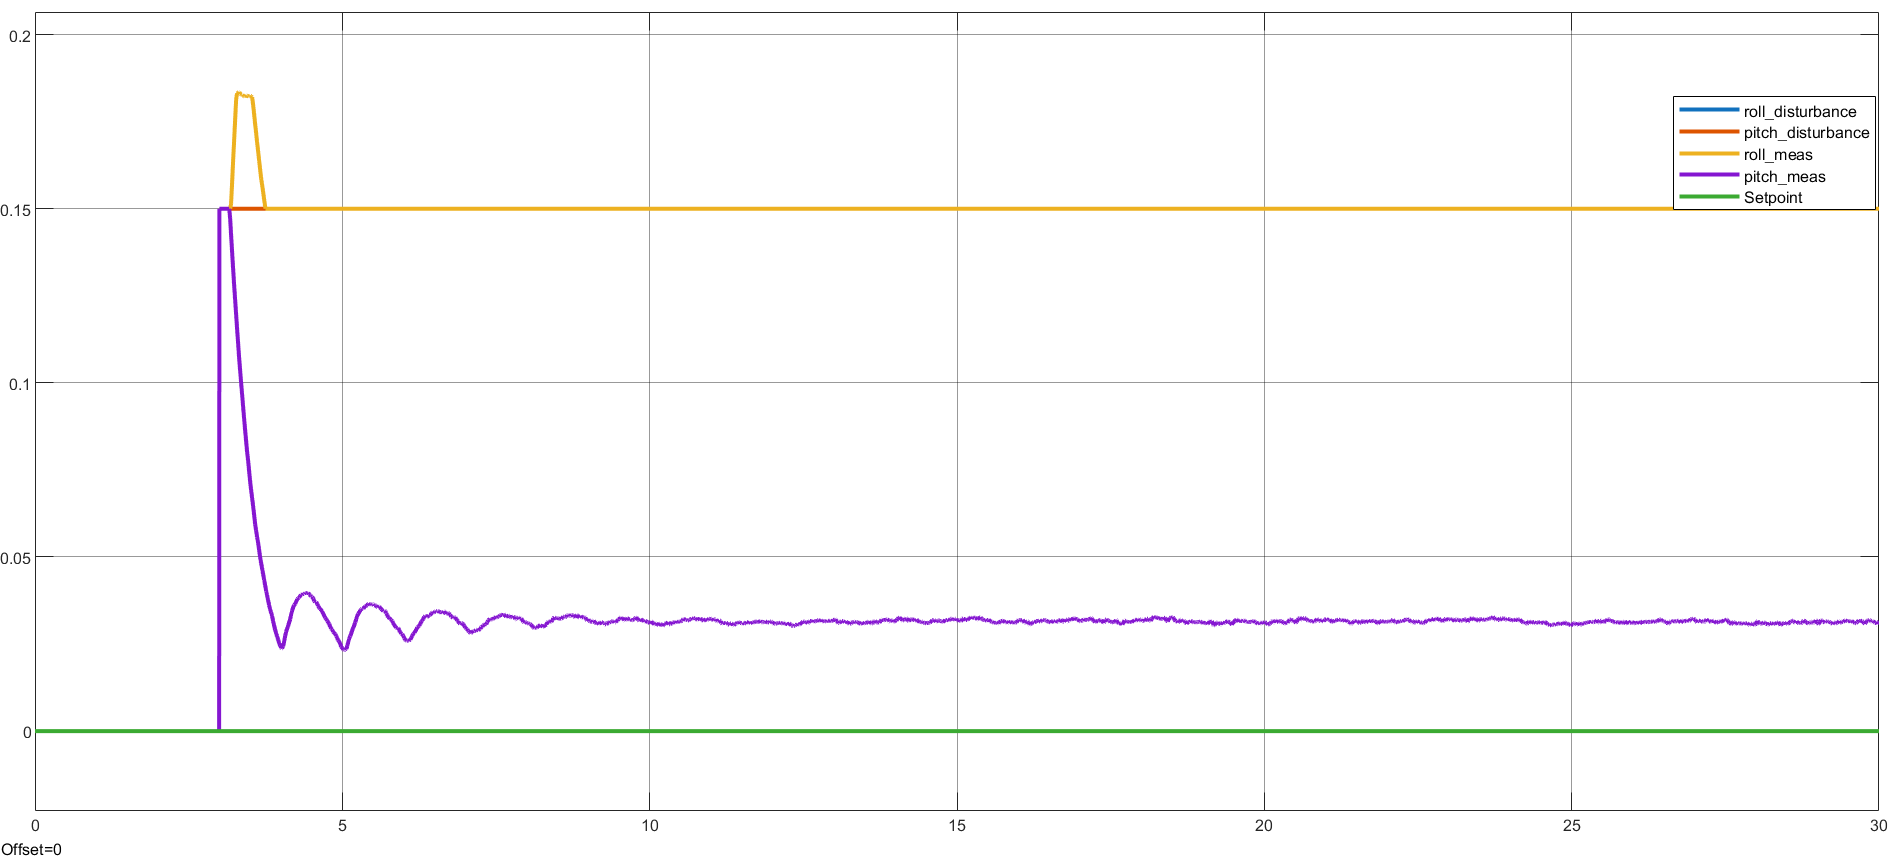
\includegraphics[width=\textwidth]{Images/PID_turning/PID_turning/pitch turning Kp=5 Kd=1.3.png}
        \caption{Dùng khâu PD ($K_p=5, K_d=1{,}3$)}
        \label{fig:pitch_tuning_pd}
    \end{subfigure}
    
    \vspace{0.2cm}
    \begin{subfigure}[b]{0.6\textwidth}
        \centering
        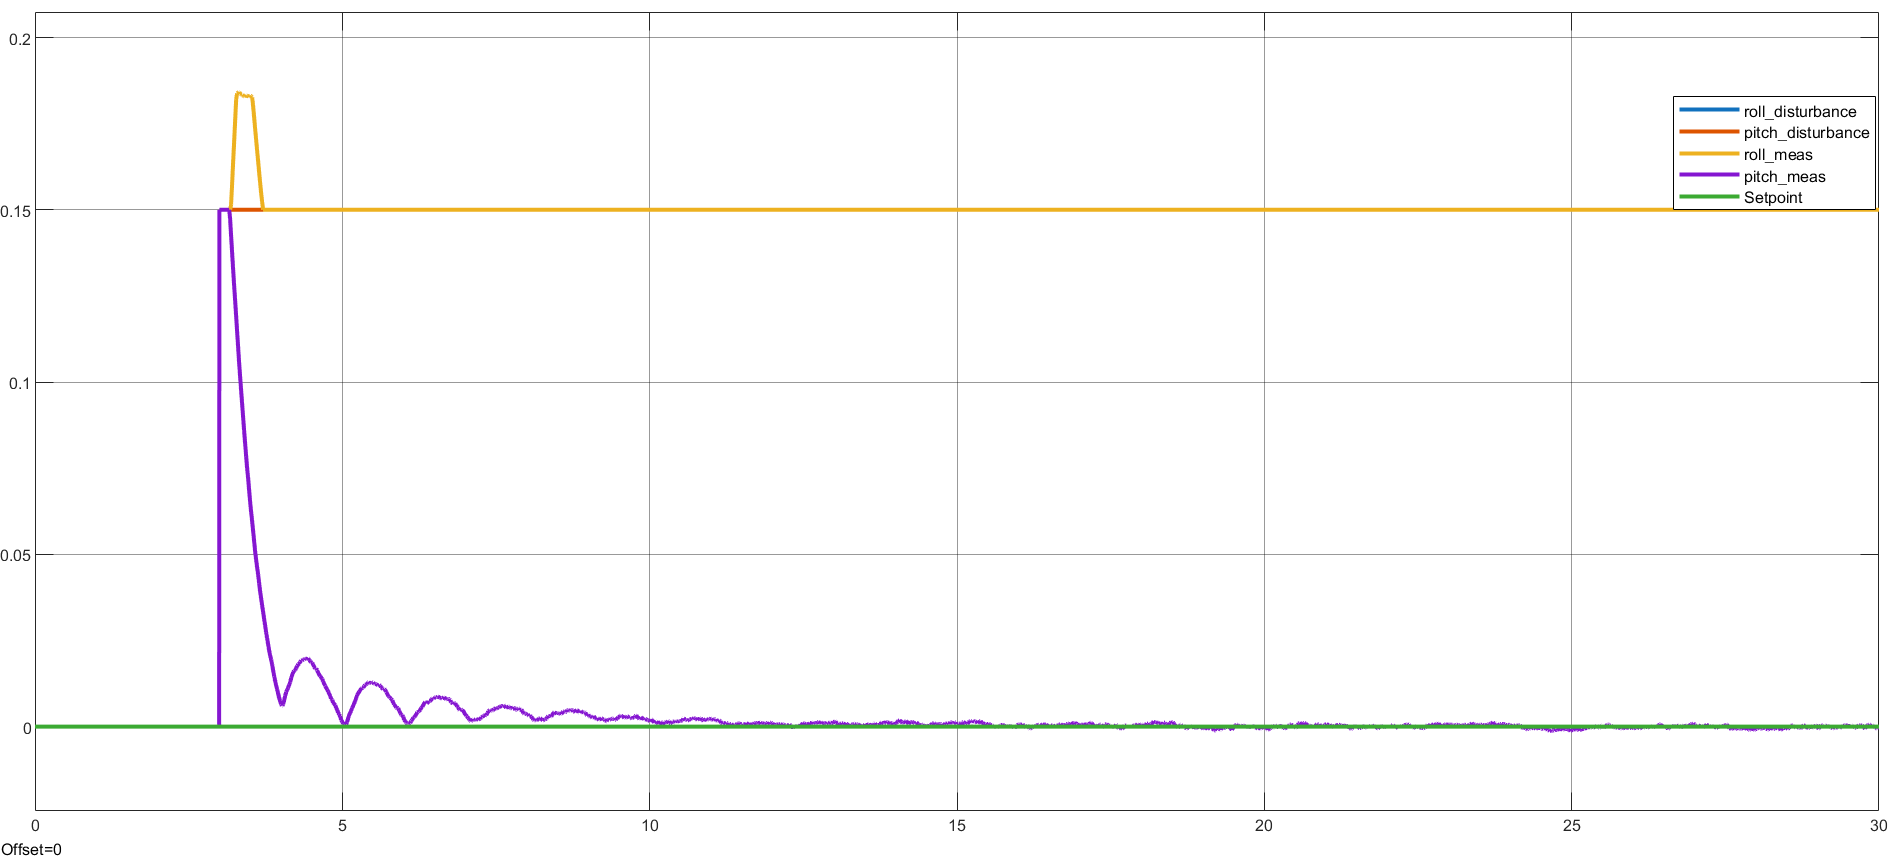
\includegraphics[width=\textwidth]{Images/PID_turning/PID_turning/pitch turning Kp=5 Kd=1.3 Ki=1.6.png}
        \caption{Dùng PID hoàn chỉnh ($K_p=5, K_i=1{,}6, K_d=1{,}3$)}
        \label{fig:pitch_tuning_pid}
    \end{subfigure}
    \caption{Quá trình hiệu chỉnh các khâu P, D, I cho trục Pitch}
    \label{fig:pitch_tuning_process}
\end{figure}

\subsubsection*{Trường hợp sử dụng bộ điều khiển PID hoàn chỉnh (sau khi Tuning)}
Để đánh giá độ ổn định tổng thể sau khi đã hiệu chỉnh, hệ thống được thử nghiệm với tín hiệu nhiễu đồng thời trên cả hai trục. Bộ thông số độc lập là Roll ($K_p=4, K_i=1{,}2, K_d=1{,}3$) và Pitch ($K_p=5, K_i=1{,}6, K_d=1{,}3$). Hình~\ref{fig:pid_noise_step} và Hình~\ref{fig:pid_noise_sine} minh họa đáp ứng của hệ thống dưới tác động của nhiễu bước (step) và nhiễu hình sin.

\begin{figure}[H]
    \centering
    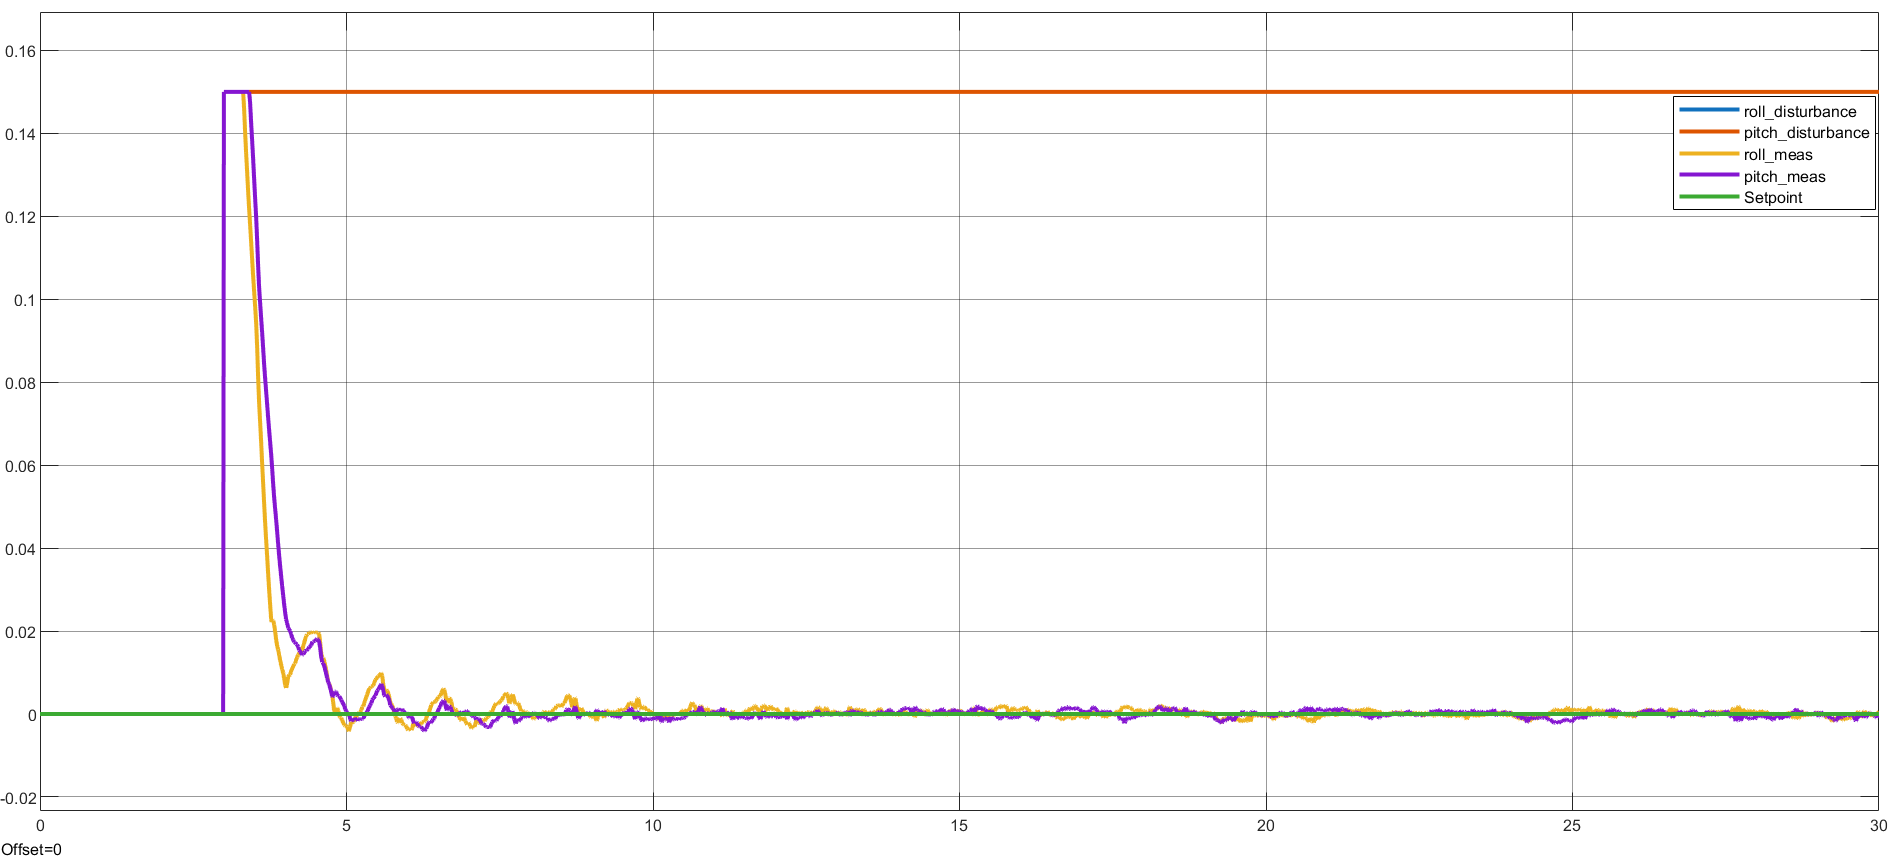
\includegraphics[width=0.8\textwidth]{Images/PID_turning/PID_turning/PID turning nhiễu step.png}
    \caption{Đồ thị đáp ứng hệ thống với tín hiệu nhiễu bước (step) trên cả 2 trục}
    \label{fig:pid_noise_step}
\end{figure}

Từ đồ thị Hình~\ref{fig:pid_noise_step}, tại thời điểm $t = 3$ s, một nhiễu bước có biên độ $0{,}15$ rad được đưa vào hệ thống. Phân tích đồ thị cho thấy ba đặc điểm nổi bật. Thứ nhất, về độ vọt lố (Overshoot), cả hai trục Roll và Pitch đều có độ vọt lố rất nhỏ; khi bù nhiễu, góc vượt qua mốc $0$, đạt giá trị âm lớn nhất khoảng $-0{,}005$ rad. Mức vọt lố này nằm trong giới hạn vô cùng an toàn, đảm bảo robot không bị mất trọng tâm dẫn đến lật ngã. Thứ hai, về thời gian quá độ (Settling Time), hệ thống mất khoảng $7-9$ s (từ $t = 3$ s đến $t = 12$ s) để dập tắt hoàn toàn các dao động và dao động tắt dần quanh giá trị cân bằng, chứng tỏ khả năng đáp ứng khá nhanh trước các thay đổi bất ngờ. Cuối cùng, về sai số xác lập (Steady-state Error), từ sau mốc $t = 12$ s, hệ thống hoàn toàn duy trì được trạng thái thăng bằng với sai số tĩnh xấp xỉ bằng $0$. Điều này minh chứng thành phần khâu tích phân (I) trong bộ điều khiển PID đã hoạt động cực kỳ hiệu quả để triệt tiêu các sai lệch dư.

\begin{figure}[H]
    \centering
    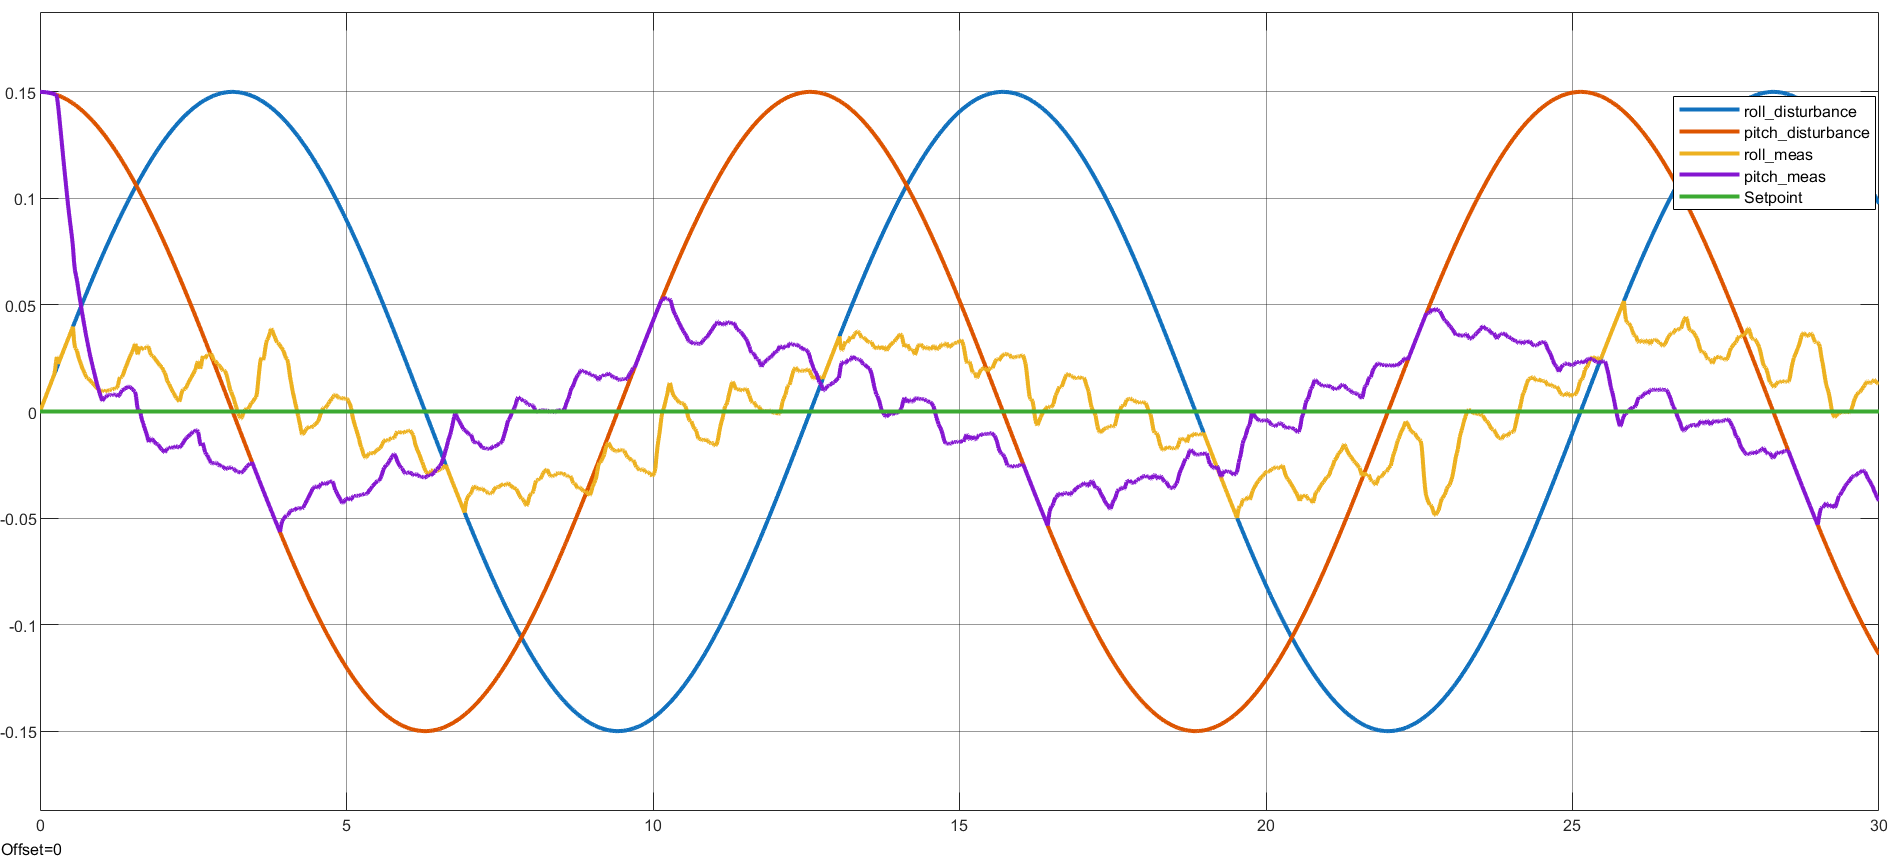
\includegraphics[width=0.8\textwidth]{Images/PID_turning/PID_turning/PID turning nhiễu sin.png}
    \caption{Đồ thị đáp ứng hệ thống với tín hiệu nhiễu hình sin trên cả 2 trục}
    \label{fig:pid_noise_sine}
\end{figure}
\textbf{\textit{Nhận xét so sánh}} 

Trong khi bộ PID có xu hướng đưa quỹ đạo nhanh chóng trở lại ổn định sau một pha "thu chân" và "duỗi chân" mạnh (tương ứng với thời điểm khâu D phản ứng mạnh với độ dốc của nhiễu), thì ở trường hợp bù trực tiếp, hiện tượng này kéo dài và có biên độ thu-duỗi thấp hơn. Sự khác biệt này phản ánh trực tiếp khả năng loại bỏ nhiễu nhanh chóng của một bộ điều khiển có khâu dự báo (D) và khâu tích lũy sai số (I) so với một hệ thống chỉ phản ứng dựa trên sai số tĩnh tại (P).


\subsubsection*{Trường hợp bù sai số trực tiếp ($K_p=1$, $K_i=0$, $K_d=0$)}
Nhằm mục đích đối chiếu hiệu quả của các khâu I và D trong bộ điều khiển PID, một mô phỏng tương tự được thực hiện với trường hợp bù sai số trực tiếp, tương đương thông số $K_p=1, K_i=0, K_d=0$.

\begin{figure}[H]
    \centering
    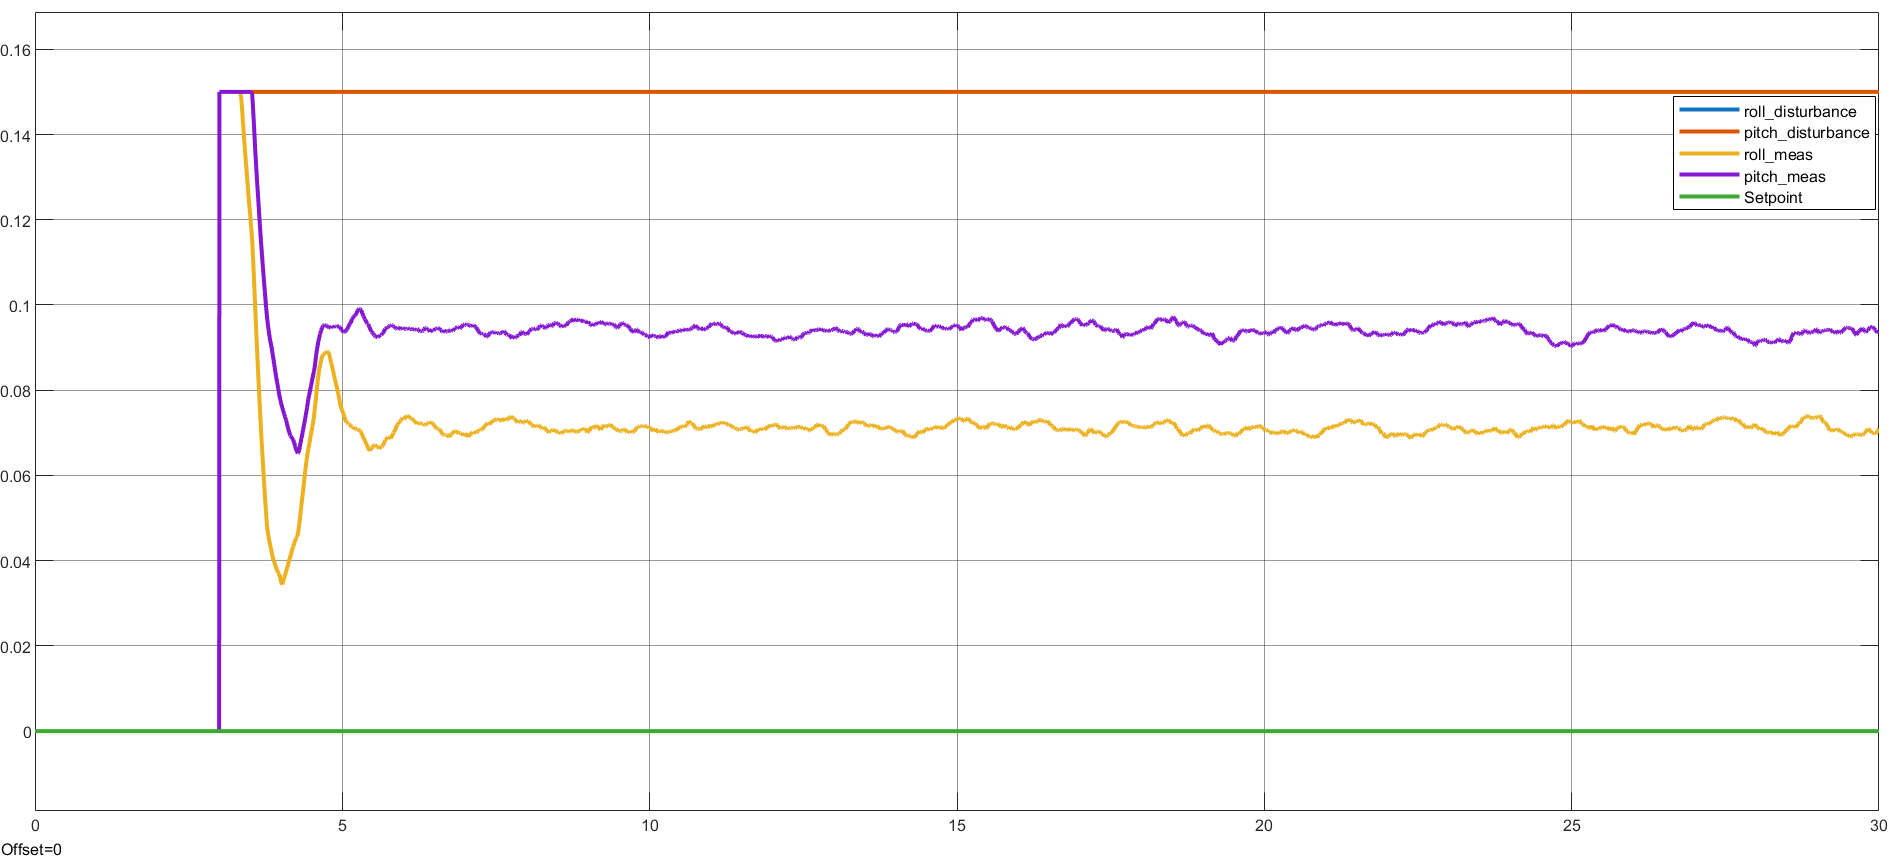
\includegraphics[width=0.8\textwidth]{Images/PID_turning/PID_turning/PID bù trực tiếp Kp=1 step.png}
    \caption{Đồ thị đáp ứng hệ thống với tín hiệu nhiễu bước (step) ($K_p=1, K_i=0, K_d=0$)}
    \label{fig:p_noise_step}
\end{figure}

Từ đồ thị Hình~\ref{fig:p_noise_step}, đồ thị biểu diễn góc nghiêng thực tế đo được (measured angle) của thân robot, khi nhiễu bước có biên độ $D = 0{,}15$ rad tác động vào hệ thống tại $t = 3$ s, thân robot bị nghiêng đi một góc tương ứng. Khảo sát đáp ứng của hệ thống trong trường hợp bù trực tiếp ($K_p=1, K_i=0, K_d=0$) cho thấy sự khác biệt rõ rệt so với bộ điều khiển PID hoàn chỉnh. Trước hết, khác với PID hoàn chỉnh, trường hợp bù trực tiếp hoàn toàn không có độ vọt lố qua mốc cân bằng $0$; góc nghiêng đo được giảm dần nhưng chưa bao giờ đạt tới hay vượt qua mốc $0$ rad. Bên cạnh đó, về dao động và thời gian quá độ, mặc dù không vượt qua mốc $0$, hệ thống lại xuất hiện trạng thái dao động (oscillatory behavior) kéo dài. Hiện tượng này xảy ra do sự vắng mặt của thành phần vi phân (D), vốn đóng vai trò dự báo và triệt tiêu sự thay đổi đột ngột của sai lệch. Hậu quả là, nếu không có khâu D, hệ thống mất hơn $15$ s để các dao động suy giảm và ổn định trở lại. Nghiêm trọng nhất là vấn đề sai số xác lập; sau thời gian quá độ, góc nghiêng xác lập ở mức khá cao, dao động quanh $0{,}07$ rad đối với Roll và $0{,}05$ rad đối với Pitch. Hệ thống vòng kín tỷ lệ 1:1 không thể bù trừ triệt để lượng nhiễu đầu vào, từ đó đòi hỏi bắt buộc phải tích hợp khâu tích phân (I) nhằm duy trì tín hiệu bù kể cả khi góc nghiêng tiến về $0$.

\begin{figure}[H]
    \centering
    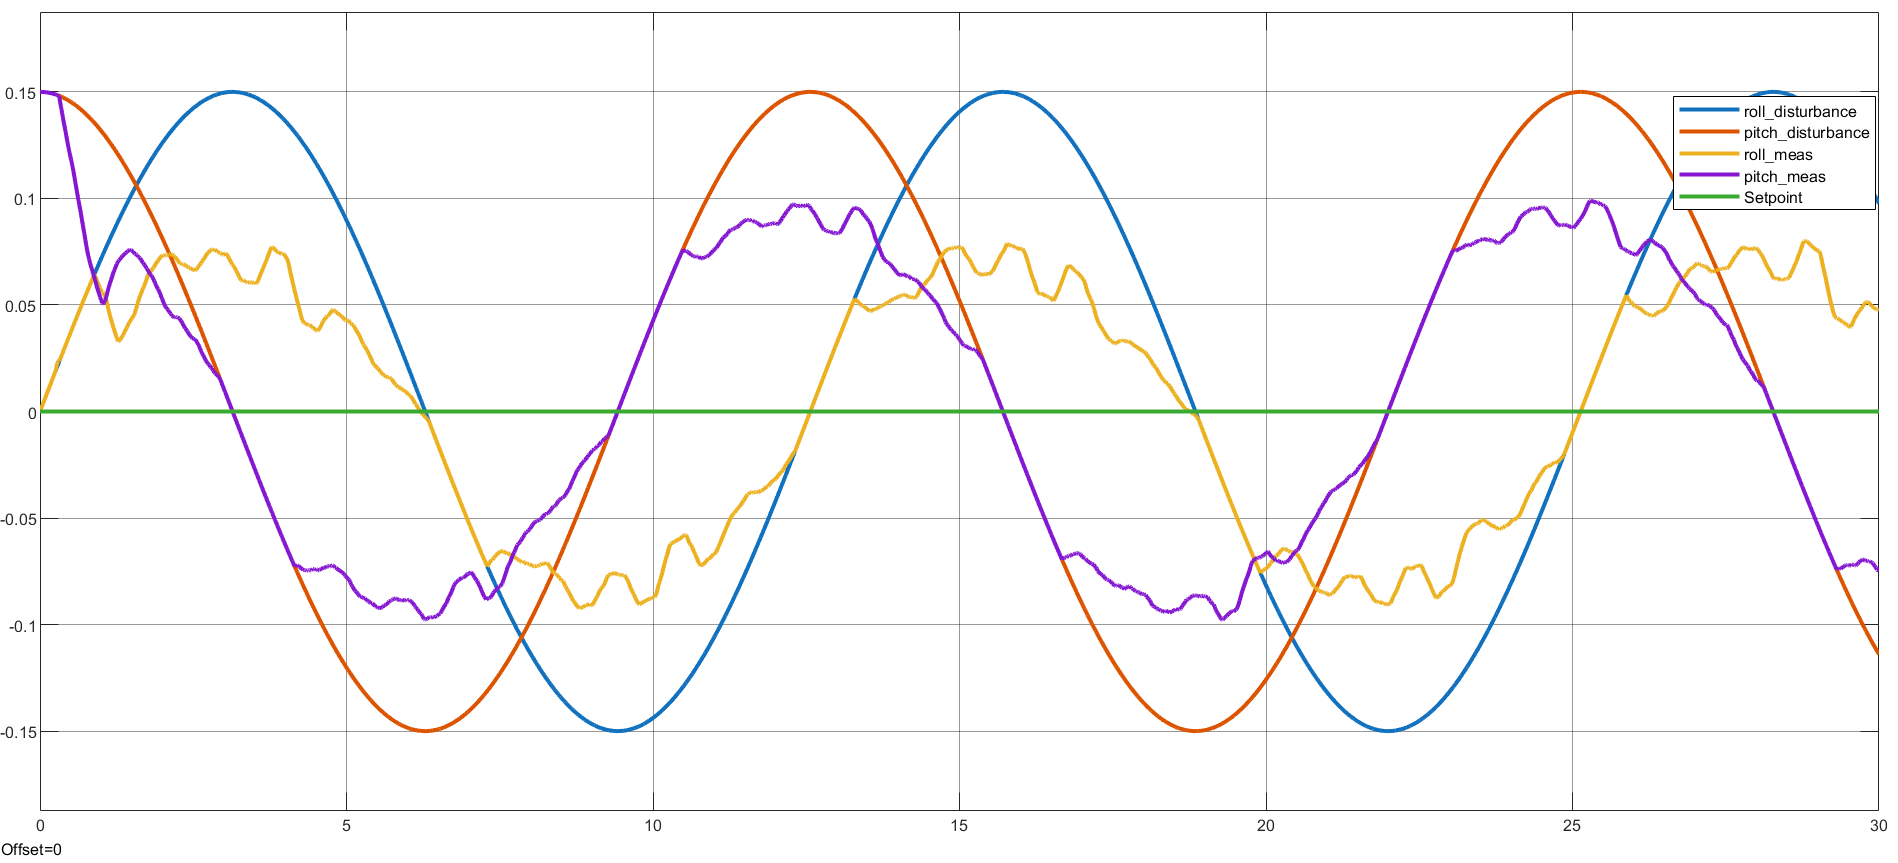
\includegraphics[width=0.8\textwidth]{Images/PID_turning/PID_turning/PID bù trực tiếp Kp=1 sin.png}
    \caption{Đồ thị đáp ứng hệ thống với tín hiệu nhiễu hình sin ($K_p=1, K_i=0, K_d=0$)}
    \label{fig:p_noise_sine}
\end{figure}

\textbf{\textit{Nhận xét so sánh}}

Thông qua việc đối chiếu giữa bộ điều khiển PID độc lập hai trục và cấu hình bù trực tiếp vòng kín ($K_p=1, K_i=0, K_d=0$), có thể khẳng định tính tất yếu của việc tuning riêng biệt các khâu I và D. Tư duy bù trực tiếp để lại sai số xác lập quá lớn và gây ra dao động kéo dài do vắng mặt khâu vi phân. Ngược lại, bộ PID hoàn chỉnh đã loại bỏ triệt để sai số xác lập, khống chế vọt lố ở mức cực nhỏ (âm $\sim 0{,}005$ rad) và xác lập tính ổn định nhanh chóng.

Các Hình~\ref{fig:pid_response_7}, Hình~\ref{fig:pid_response_8} và Hình~\ref{fig:pid_response_9} trình bày các tín hiệu nội bộ thu được trong quá trình mô phỏng khi robot thực hiện chu trình di chuyển có tính tuần hoàn (dáng đi Trot).

Hình~\ref{fig:pid_response_7} thể hiện quỹ đạo tọa độ trục Z (\texttt{z\_out}) của 4 bàn chân robot theo thời gian, cho thấy sự kết hợp giữa quỹ đạo bước đi cơ sở và tín hiệu bù từ bộ điều khiển PID. Cụ thể, trước thời điểm $t = 3$ s, cả 4 chân đều có chung một biên dạng ổn định, trong đó pha chống chân nằm ở mức âm cơ sở, và pha vung chân tạo thành các đỉnh nhọn nhấc lên đều đặn. Tuy nhiên, từ thời điểm $t = 3$ s, khi nhiễu nghiêng xuất hiện, đồ thị bắt đầu phân hóa rõ rệt với đường cơ sở nhảy vọt và các đỉnh vung chân hướng xuống mạnh mẽ. Hiện tượng này được giải thích bởi nguyên lý động học (Kinematic Coupling): sự cộng hưởng của nhiễu Roll và Pitch khi robot bị nghiêng mạnh khiến một số điểm chân bị ép sát xuống mặt đất nhất. Để bù trừ, PID ra lệnh thu chân lại cực hạn. Trong tư thế gập sâu này, kết hợp với việc hệ trục tọa độ thân robot đã bị nghiêng lớn, động tác vung chân về phía trước bị "khớp nối động học" và chuyển hóa thành chuyển động duỗi dài ra theo trục Z của thân robot để có thể chạm tới điểm đặt chân mong muốn. Chuỗi phản ứng này minh họa rõ rệt giới hạn không gian làm việc (workspace boundary) và tính chất phức tạp của robot bốn chân dưới tác động của sai lệch tư thế lớn.

\begin{figure}[H]
    \centering
    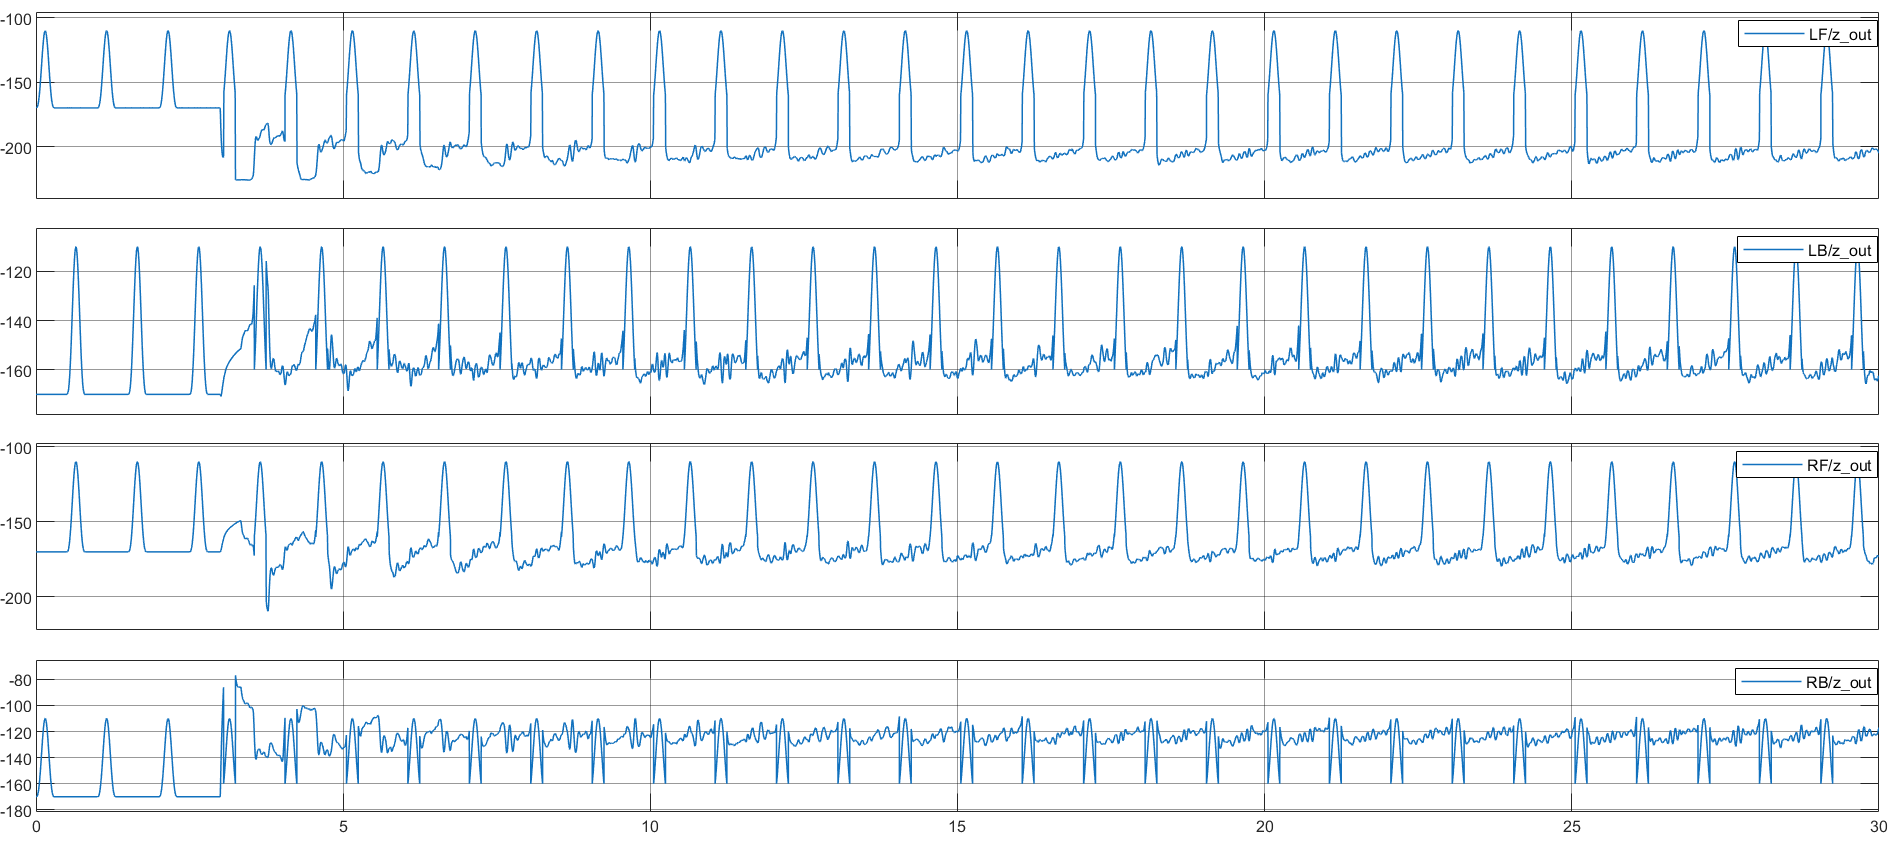
\includegraphics[width=0.8\textwidth]{Images/PID_turning/PID_turning/zout.png}
    \caption{Đồ thị tín hiệu vị trí cao độ bàn chân trục Z (\texttt{z\_out}) của 4 chân robot}
    \label{fig:pid_response_7}
\end{figure}

Các Hình~\ref{fig:pid_response_8} và Hình~\ref{fig:pid_response_9} minh họa quá trình tiền xử lý tín hiệu bên trong bộ điều khiển PID góc Roll và Pitch nhằm phân lập sai lệch tư thế khỏi các dao động sinh ra do chu trình bước đi. Quá trình bắt đầu với tín hiệu \texttt{roll\_meas} và \texttt{pitch\_meas}, vốn bao gồm các dao động tuần hoàn biên độ lớn do sự dịch chuyển trọng tâm luân phiên giữa các chân. Tín hiệu này sau đó đi qua bộ lọc trung bình trượt hàm mũ (EMA) để làm suy giảm các nhiễu rung động cơ học tần số cao do va đập, giúp bảo toàn sóng cơ bản của dáng đi. Tiếp đến, bộ lọc trung bình (Avg) đóng vai trò then chốt như một bộ lọc thông thấp (Low-pass Filter). Ví dụ tại $t = 3$ s, khi nhiễu bước tác động vào hệ thống, bộ lọc Avg đã triệt tiêu phần lớn dao động của dáng đi và trích xuất thành công độ trôi dạt tư thế (baseline drift). Cuối cùng, tín hiệu đi qua khâu vùng chết (Deadzone) để cắt xén phần vi sai dư thừa, minh chứng rằng bộ điều khiển đã trích xuất được mức sai số tư thế hữu ích và chính xác nhằm đưa vào khâu tính toán PID, qua đó loại bỏ hoàn toàn hiện tượng phản ứng quá mức với các dao động tự nhiên.
Dựa trên chuỗi tín hiệu đã được xử lý này, bộ điều khiển PID tính toán phản hồi chuẩn xác mà không phá vỡ động học di chuyển tự nhiên của robot.

\begin{figure}[H]
    \centering
    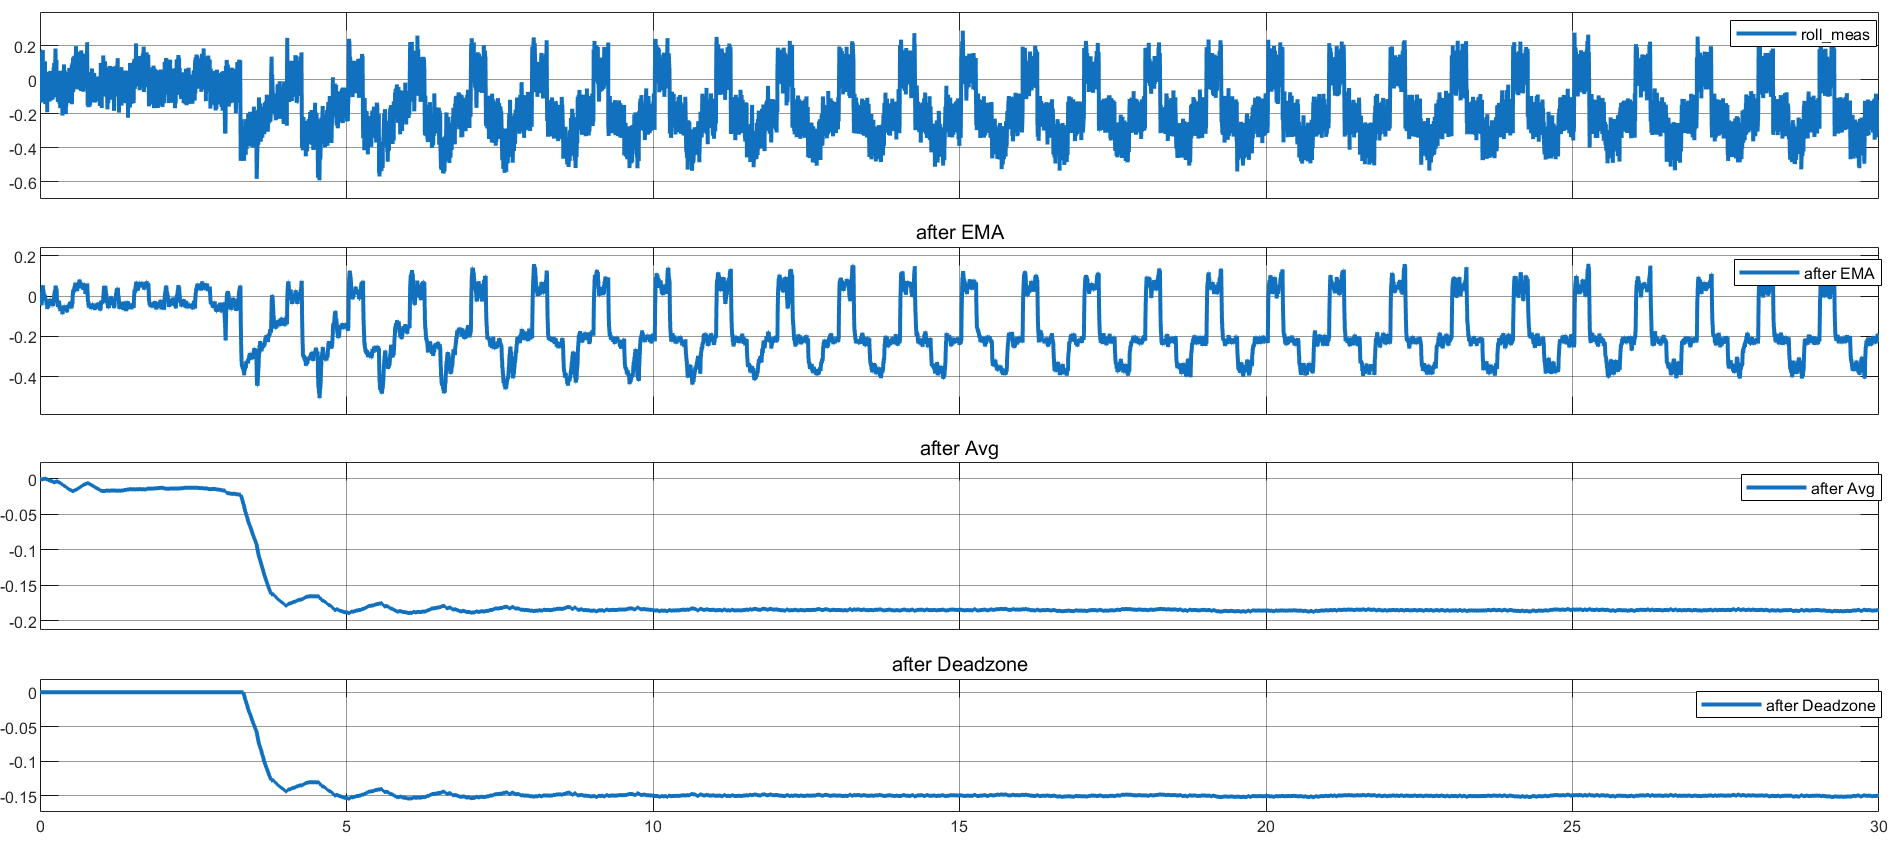
\includegraphics[width=0.8\textwidth]{Images/PID_turning/PID_turning/xử lí roll trước khi đưa vào PID.png}
    \caption{Đồ thị các tín hiệu xử lý nội bộ của bộ điều khiển PID góc Roll}
    \label{fig:pid_response_8}
\end{figure}

\begin{figure}[H]
    \centering
    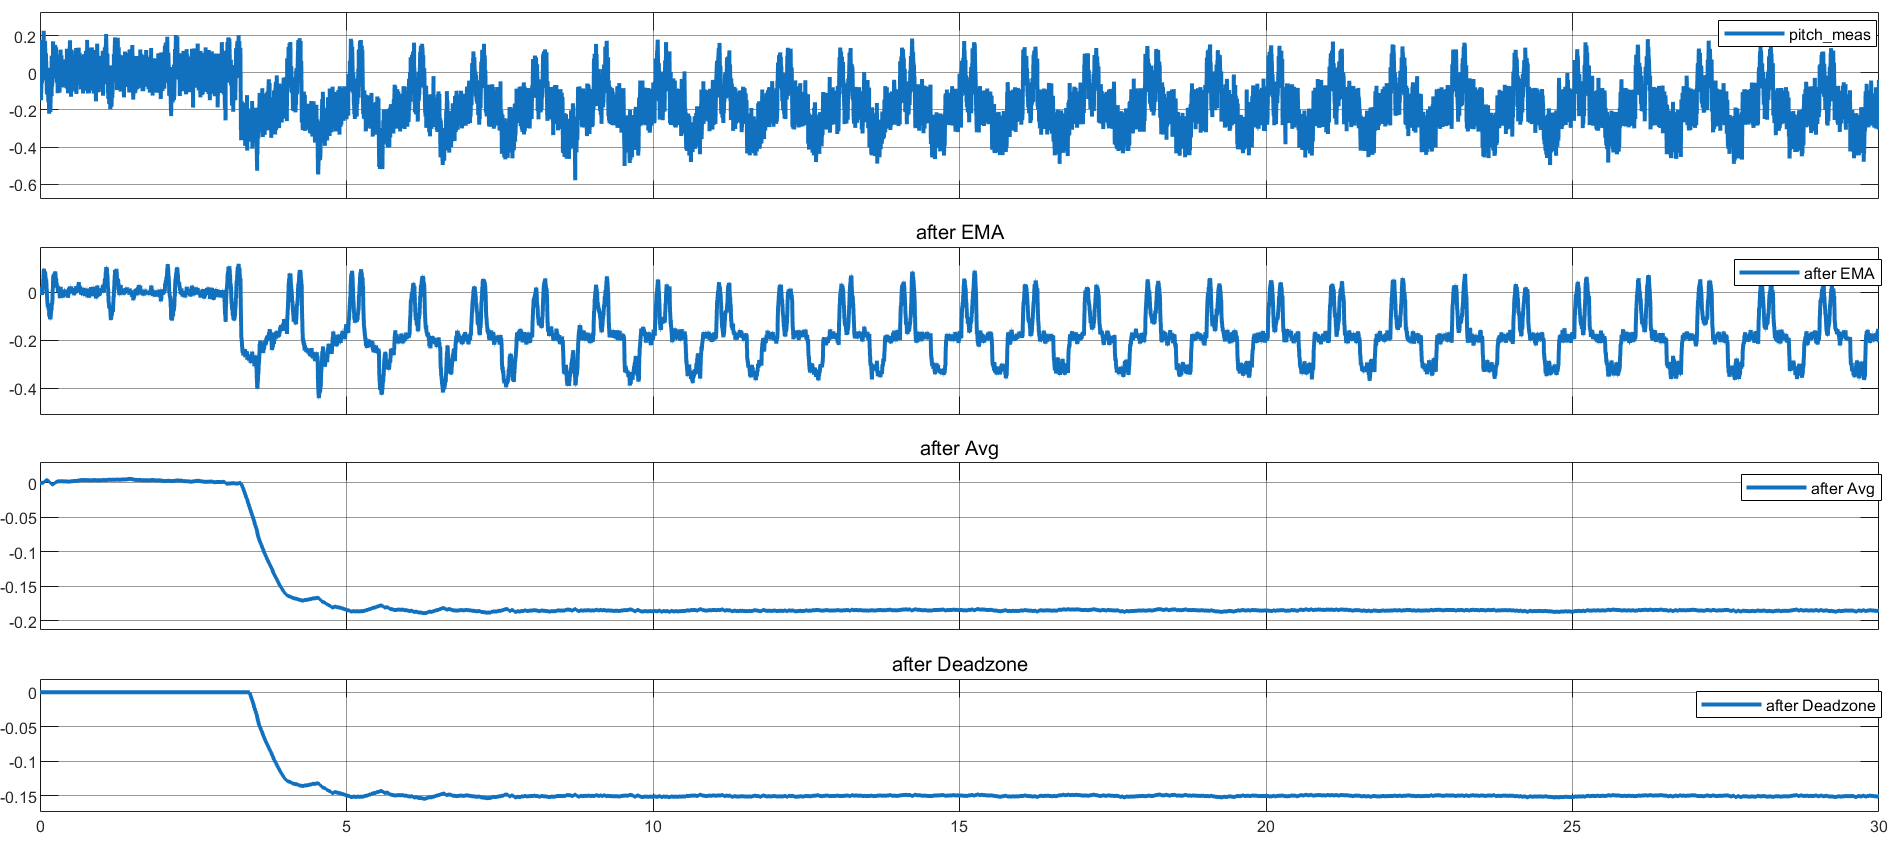
\includegraphics[width=0.8\textwidth]{Images/PID_turning/PID_turning/xử lí pitch trước khi đưa vào PID.png}
    \caption{Đồ thị các tín hiệu xử lý nội bộ của bộ điều khiển PID góc Pitch}
    \label{fig:pid_response_9}
\end{figure}

\section{Cấu hình môi trường mô phỏng Gazebo}

\subsection{Mô hình robot URDF}

Robot bốn chân được mô tả bằng file URDF (Unified Robot Description Format), định nghĩa đầy đủ cấu trúc cơ khí bao gồm 13 link (1 thân + 12 khâu chân) và 12 khớp quay (revolute joint). Mỗi link được gán các thuộc tính quán tính (khối lượng $m$, ma trận quán tính $I$), hình dạng va chạm (collision geometry) và hình dạng hiển thị (visual geometry) sử dụng file mesh STL.

Các tham số hình học chính của mô hình URDF được trình bày trong Bảng~\ref{tab:urdf_params}.

\begin{table}[H]
\centering
\caption{Tham số hình học mô hình URDF}
\label{tab:urdf_params}
\renewcommand{\arraystretch}{1.3}
\begin{tabular}{|l|c|c|l|}
\hline
\textbf{Tham số} & \textbf{Ký hiệu} & \textbf{Giá trị} & \textbf{Đơn vị} \\ \hline
Chiều dài thân & $L$ & 209 & mm \\ \hline
Chiều rộng thân & $W$ & 191 & mm \\ \hline
Chiều dài khớp coxa & $l_1$ & 26 & mm \\ \hline
Chiều dài xương đùi & $l_2$ & 106 & mm \\ \hline
Chiều dài xương ống chân & $l_3$ & 125 & mm \\ \hline
Khối lượng thân & $m_{body}$ & 1,5 & kg \\ \hline
Khối lượng mỗi link chân & $m_{leg}$ & 0,05--0,15 & kg \\ \hline
Giới hạn effort khớp hip & $\tau_{max,hip}$ & 2,94 & Nm \\ \hline
Giới hạn effort khớp tibia & $\tau_{max,tibia}$ & 1,96 & Nm \\ \hline
\end{tabular}
\end{table}

Kích thước URDF trong mô phỏng được cập nhật để khớp hoàn toàn với robot thực tế ($L=209$ mm, $W=191$ mm, $l_1=26$ mm, $l_2=106$ mm, $l_3=125$ mm). Điều này đảm bảo tính nhất quán cao nhất giữa mô phỏng và phần cứng.

\subsection{Plugin điều khiển Gazebo}

Giao diện điều khiển giữa ROS~2 và Gazebo sử dụng plugin \texttt{gazebo\_ros2\_control} với cấu hình effort command interface. Trong chế độ này, ROS~2 gửi giá trị mô-men xoắn (effort, đơn vị Nm) trực tiếp đến các khớp trong Gazebo, thay vì gửi vị trí hoặc vận tốc. Bộ điều khiển PD cấp thấp được triển khai phía ROS~2 để chuyển đổi sai lệch vị trí thành mô-men:

\begin{equation}
    \tau_i = K_p (\theta_{target,i} - \theta_{actual,i}) - K_d \cdot \omega_{actual,i}
\end{equation}

trong đó $\theta_{target,i}$ là góc mong muốn từ IK, $\theta_{actual,i}$ và $\omega_{actual,i}$ là vị trí và vận tốc góc thực tế đọc từ Gazebo.

\subsection{Cấu hình vật lý và môi trường}

Môi trường mô phỏng được cấu hình chặt chẽ với các tham số vật lý chuyên dụng. Hệ thống sử dụng engine vật lý ODE (Open Dynamics Engine) chạy ở bước thời gian $\Delta t = 1$ ms, tương đương tần số 1000 Hz. Trọng lực được thiết lập ở mức chuẩn $g = 9{,}81$ m/s$^2$ tác dụng theo phương $-z$, kết hợp với mặt phẳng đất vô hạn tại $z = 0$ (không có địa hình nhấp nhô) và có hệ số ma sát Coulomb $\mu = 0{,}8$ nhằm mô phỏng bề mặt nhám. Ngoài ra, cảm biến IMU ảo được tích hợp thông qua plugin \texttt{libgazebo\_ros\_imu\_sensor.so}, chịu trách nhiệm cung cấp dữ liệu quaternion, vận tốc góc và gia tốc tuyến tính tại tần số 100 Hz. Cảm biến này cũng được thêm nhiễu Gaussian, cụ thể $\sigma = 0{,}001$ rad/s đối với con quay hồi chuyển và $\sigma = 0{,}01$ m/s$^2$ đối với gia tốc kế, nhằm phản ánh chính xác các giới hạn của cảm biến vật lý.

Tốc độ cập nhật bộ điều khiển ROS~2 được đặt ở 1000 Hz ($f_{ctrl} = 1000$ Hz), đồng bộ với bước thời gian vật lý của Gazebo. Chu kỳ timer của Gait Generator node là 3 ms, tương ứng với tần số xuất lệnh quỹ đạo 333 Hz.

\subsection{Kết quả mô phỏng vận động cơ bản}

Sau khi cấu hình xong môi trường, các thử nghiệm vận động cơ bản được tiến hành trên Gazebo để đánh giá khả năng di chuyển động học trước khi phân tích sâu vào hệ thống điều khiển.

Hình \ref{fig:sim_home} minh họa chuỗi hình ảnh quá trình khởi tạo tư thế đứng chuẩn của robot từ lúc khởi động trên hệ thống mô phỏng Gazebo.

\begin{figure}[H]
    \centering
    \begin{subfigure}[b]{0.19\textwidth}
        
\includegraphics[width=\textwidth]{real_robot/gait/frames_cropped/1.jpg}
        \caption{$t=0.1$ s}
    \end{subfigure}
    \hfill
    \begin{subfigure}[b]{0.19\textwidth}
        
\includegraphics[width=\textwidth]{real_robot/gait/frames_cropped/2.jpg}
        \caption{$t=0.2$ s}
    \end{subfigure}
    \hfill
    \begin{subfigure}[b]{0.19\textwidth}
        
\includegraphics[width=\textwidth]{real_robot/gait/frames_cropped/3.jpg}
        \caption{$t=0.3$ s}
    \end{subfigure}
    \hfill
    \begin{subfigure}[b]{0.19\textwidth}
        
\includegraphics[width=\textwidth]{real_robot/gait/frames_cropped/4.jpg}
        \caption{$t=0.4$ s}
    \end{subfigure}
    \hfill
    \begin{subfigure}[b]{0.19\textwidth}
        
\includegraphics[width=\textwidth]{real_robot/gait/frames_cropped/5.jpg}
        \caption{$t=0.5$ s}
    \end{subfigure}
    
    \vspace{0.2cm}
    \begin{subfigure}[b]{0.19\textwidth}
        
\includegraphics[width=\textwidth]{real_robot/gait/frames_cropped/6.jpg}
        \caption{$t=0.6$ s}
    \end{subfigure}
    \hfill
    \begin{subfigure}[b]{0.19\textwidth}
        
\includegraphics[width=\textwidth]{real_robot/gait/frames_cropped/7.jpg}
        \caption{$t=0.7$ s}
    \end{subfigure}
    \hfill
    \begin{subfigure}[b]{0.19\textwidth}
        
\includegraphics[width=\textwidth]{real_robot/gait/frames_cropped/8.jpg}
        \caption{$t=0.8$ s}
    \end{subfigure}
    \hfill
    \begin{subfigure}[b]{0.19\textwidth}
        
\includegraphics[width=\textwidth]{real_robot/gait/frames_cropped/9.jpg}
        \caption{$t=0.9$ s}
    \end{subfigure}
    \hfill
    \begin{subfigure}[b]{0.19\textwidth}
        
\includegraphics[width=\textwidth]{real_robot/gait/frames_cropped/10.jpg}
        \caption{$t=1.0$ s}
    \end{subfigure}
    \caption{Chuỗi chuyển động quá trình khởi tạo tư thế đứng của robot trên mô phỏng Gazebo.}
    \label{fig:sim_home}
\end{figure}


Hình \ref{fig:sim_trot_sequence} ghi lại chuỗi hình ảnh của robot khi thực hiện dáng đi Trot trên hệ thống mô phỏng Gazebo. Các pha luân phiên nhấc chân và chống chân được thể hiện rõ ràng.

\begin{figure}[H]
    \centering
    \begin{subfigure}[b]{0.19\textwidth}
        
\includegraphics[width=\textwidth]{real_robot/gait/frames_cropped/20.jpg}
        \caption{$t=2.0$ s}
    \end{subfigure}
    \hfill
    \begin{subfigure}[b]{0.19\textwidth}
        
\includegraphics[width=\textwidth]{real_robot/gait/frames_cropped/30.jpg}
        \caption{$t=3.0$ s}
    \end{subfigure}
    \hfill
    \begin{subfigure}[b]{0.19\textwidth}
        
\includegraphics[width=\textwidth]{real_robot/gait/frames_cropped/40.jpg}
        \caption{$t=4.0$ s}
    \end{subfigure}
    \hfill
    \begin{subfigure}[b]{0.19\textwidth}
        
\includegraphics[width=\textwidth]{real_robot/gait/frames_cropped/50.jpg}
        \caption{$t=5.0$ s}
    \end{subfigure}
    \hfill
    \begin{subfigure}[b]{0.19\textwidth}
        
\includegraphics[width=\textwidth]{real_robot/gait/frames_cropped/60.jpg}
        \caption{$t=6.0$ s}
    \end{subfigure}
    
    \vspace{0.2cm}
    \begin{subfigure}[b]{0.19\textwidth}
        
\includegraphics[width=\textwidth]{real_robot/gait/frames_cropped/70.jpg}
        \caption{$t=7.0$ s}
    \end{subfigure}
    \hfill
    \begin{subfigure}[b]{0.19\textwidth}
        
\includegraphics[width=\textwidth]{real_robot/gait/frames_cropped/80.jpg}
        \caption{$t=8.0$ s}
    \end{subfigure}
    \hfill
    \begin{subfigure}[b]{0.19\textwidth}
        
\includegraphics[width=\textwidth]{real_robot/gait/frames_cropped/90.jpg}
        \caption{$t=9.0$ s}
    \end{subfigure}
    \hfill
    \begin{subfigure}[b]{0.19\textwidth}
        
\includegraphics[width=\textwidth]{real_robot/gait/frames_cropped/100.jpg}
        \caption{$t=10.0$ s}
    \end{subfigure}
    \hfill
    \begin{subfigure}[b]{0.19\textwidth}
        
\includegraphics[width=\textwidth]{real_robot/gait/frames_cropped/110.jpg}
        \caption{$t=11.0$ s}
    \end{subfigure}
    \caption{Chuỗi chuyển động của robot trên hệ thống mô phỏng trong dáng đi Trot.}
    \label{fig:sim_trot_sequence}
\end{figure}



\section{Đánh giá hiệu năng bộ điều khiển PID nâng cao trên mô phỏng}

Phần này trình bày các kết quả thu được từ hệ thống mô phỏng, bao gồm dữ liệu chẩn đoán từ chuỗi xử lý PID và các biên dạng quỹ đạo offline. Bảng~\ref{tab:pid_home_params} và Bảng~\ref{tab:pid_gait_params} tổng hợp toàn bộ tham số điều khiển cho hai chế độ hoạt động, được trích xuất trực tiếp từ mã nguồn hệ thống.

\begin{table}[H]
\centering
\caption{Tham số bộ điều khiển PID -- Chế độ tĩnh (HOME)}
\label{tab:pid_home_params}
\renewcommand{\arraystretch}{1.3}
\begin{tabular}{|l|c|c|l|}
\hline
\textbf{Tham số} & \textbf{Ký hiệu} & \textbf{Giá trị} & \textbf{Mô tả} \\ \hline
Hệ số tỷ lệ & $K_P$ & 2,0 & Khuếch đại sai lệch \\ \hline
Hệ số tích phân & $K_I$ & 0,30 & Triệt tiêu sai số xác lập \\ \hline
Hệ số vi phân & $K_D$ & 0,15 & Giảm chấn dao động \\ \hline
Bão hòa đầu ra & $u_{max}$ & 1,5 rad & Giới hạn tín hiệu hiệu chỉnh \\ \hline
Bão hòa tích phân & $\mathcal{I}_{max}$ & 1,5 & Chống windup \\ \hline
Rò rỉ tích phân & $\lambda$ & 0,9995 & Hệ số decay \\ \hline
Vùng chết đo & $d$ & 0,02 rad & Triệt nhiễu nhỏ \\ \hline
Ngưỡng gain schedule & $e_{thresh}$ & 0,08 rad & Ngưỡng tỷ lệ khuếch đại \\ \hline
Hệ số LPF đầu vào & $\alpha_{raw}$ & 0,4 & Lọc EMA tín hiệu thô \\ \hline
Hệ số LPF đạo hàm & $\alpha_d$ & 0,7 & Lọc thành phần D \\ \hline
Hệ số LPF đầu ra & $\alpha_c$ & 0,15 & Làm mượt tín hiệu bù \\ \hline
\end{tabular}
\end{table}

\begin{table}[H]
\centering
\caption{Tham số bộ điều khiển PID -- Chế độ động (GAIT)}
\label{tab:pid_gait_params}
\renewcommand{\arraystretch}{1.3}
\begin{tabular}{|l|c|c|l|}
\hline
\textbf{Tham số} & \textbf{Ký hiệu} & \textbf{Giá trị} & \textbf{Mô tả} \\ \hline
Hệ số tỷ lệ & $K_P$ & 3,0 & Khuếch đại động \\ \hline
Hệ số tích phân & $K_I$ & 0,005 & Rất nhỏ (tránh dao động) \\ \hline
Hệ số vi phân & $K_D$ & 1,2 & Giảm chấn mạnh \\ \hline
Hệ số động P & $K_{prop}$ & 10,0 & Chia tỷ lệ dynamic gain \\ \hline
Vùng chết trung bình & $d_{avg}$ & 0,03 rad & Ngưỡng triệt nhiễu \\ \hline
Bão hòa đầu ra & $u_{max}$ & 0,30 rad & Giới hạn nhỏ hơn HOME \\ \hline
Bão hòa tích phân & $\mathcal{I}_{max}$ & 0,3 & Chống windup \\ \hline
Hệ số LPF đầu ra & $\alpha_{lpf}$ & 0,97 & Lọc mạnh hơn HOME \\ \hline
Số chu kỳ học baseline & $N_{learn}$ & 2 & Chu kỳ dáng đi \\ \hline
Tốc độ hội tụ baseline & $\eta_{adapt}$ & 0,05 & Cập nhật baseline \\ \hline
\end{tabular}
\end{table}

Sự khác biệt giữa hai bộ tham số phản ánh yêu cầu vận hành riêng biệt: chế độ HOME cần phản ứng nhanh ($K_P = 2{,}0$, $\alpha_c = 0{,}15$) để bù nhiễu loạn tức thời, trong khi chế độ GAIT cần lọc mạnh ($\alpha_{lpf} = 0{,}97$) và giới hạn đầu ra nhỏ ($u_{max} = 0{,}30$ rad) để tránh can thiệp quá mức vào quỹ đạo sải bước.

\subsection{Kết quả quy hoạch quỹ đạo offline}

Hình~\ref{results/offline_traj_pos} trình bày quỹ đạo Cartesian $(x, y, z)$ của chân trước bên trái (Left-Front) trong một chu kỳ dáng đi đầy đủ. Việc quy hoạch quỹ đạo trục $z$ theo biên dạng parabol với độ cao $h_{lift} = 80$ mm là đặc biệt quan trọng để tạo ra hình dáng chữ D (D-shape trajectory). Thiết kế này giải quyết bài toán tránh va chạm (ground clearance), giúp chân robot không bị vấp phải các chướng ngại vật nhỏ trên mặt đất khi vung chân. Đồng thời, việc trục $y$ được duy trì ổn định tại giá trị $0$ mang ý nghĩa đảm bảo chân bước thẳng, loại bỏ hoàn toàn hiện tượng trượt ngang (slippage) -- nguyên nhân chính gây hao hụt động năng và làm suy giảm khả năng định hướng khi robot di chuyển.

\begin{figure}[H]
    \centering
    
\includegraphics[width=0.8\textwidth]{results/offline_traj_pos.png}
    \caption{Quỹ đạo Cartesian $(x, y, z)$ của chân trước bên trái trong một chu kỳ dáng đi}
    \label{results/offline_traj_pos}
\end{figure}

Hình~\ref{results/offline_traj_vel_acc} trình bày biên dạng vận tốc và gia tốc của quỹ đạo. Kết quả này không chỉ xác nhận tính đúng đắn về mặt toán học mà còn mang ý nghĩa cơ khí thiết thực: việc đáp ứng được các điều kiện biên $\dot{s}(0) = \dot{s}(1) = 0$ và $\ddot{s}(0) = \ddot{s}(1) = 0$ của hàm đa thức bậc 5 (quintic) giúp triệt tiêu hoàn toàn sự thay đổi gia tốc đột ngột (infinite jerk). Phương pháp này giải quyết bài toán chống sốc cơ học tại hai thời điểm nhạy cảm nhất là nhấc chân (lift-off) và chạm đất (touch-down), từ đó giảm thiểu hao mòn bánh răng và kéo dài tuổi thọ của các động cơ servo.

\begin{figure}[H]
    \centering
    
\includegraphics[width=0.8\textwidth]{results/offline_traj_vel_acc.png}
    \caption{Biên dạng vận tốc và gia tốc của chân trước bên trái}
    \label{results/offline_traj_vel_acc}
\end{figure}

Hình~\ref{results/offline_traj_angle} cho thấy các góc khớp $(\theta_1, \theta_2, \theta_3)$ thu được từ bộ giải động học nghịch (IK). Tính trơn tru, liên tục và không xuất hiện các đỉnh nhọn (bước nhảy) trong đồ thị này có ý nghĩa khẳng định rằng bộ tham số không gian cấu hình ($L_{stride}=10$ mm, $h_{lift}=80$ mm) được chọn nằm hoàn toàn bên trong vùng không gian làm việc an toàn (reachable workspace) của robot. Điều này chứng minh thuật toán IK đã giải quyết thành công bài toán nội suy tọa độ mà không vướng phải các điểm kỳ dị (singularities).

\begin{figure}[H]
    \centering
    
\includegraphics[width=0.8\textwidth]{results/offline_traj_angle.png}
    \caption{Góc khớp $(\theta_1, \theta_2, \theta_3)$ giải qua IK cho các chân bên trái (LF và LB)}
    \label{results/offline_traj_angle}
\end{figure}

\subsection{Quỹ đạo 3D bàn chân trong môi trường mô phỏng}

Hình~\ref{fig_gait_3d_real} trình bày quỹ đạo 3D thực tế của bàn chân khi chạy trong môi trường mô phỏng Gazebo. Ý nghĩa của đồ thị này vượt ra ngoài việc xác nhận hình chữ D đặc trưng; nó minh chứng cho sự tương thích hoàn hảo giữa luồng phần mềm lập kế hoạch tĩnh (ROS~2 node) và Engine vật lý động lực học (chịu ảnh hưởng của trọng lực, ma sát, quán tính). Quỹ đạo thực tế bám sát quỹ đạo lý thuyết chứng minh rằng bộ điều khiển cấp thấp (Low-level PD controller) trên mô phỏng đã giải quyết tốt bài toán thực thi quỹ đạo dưới tải trọng ảo của robot.

\begin{figure}[H]
    \centering
    
\includegraphics[width=0.6\textwidth]{gait_planner/gait_3d.png}
    \caption{Quỹ đạo 3D bàn chân chân trước bên trái trên hệ thống mô phỏng}
    \label{fig_gait_3d_real}
\end{figure}

\subsection{Ổn định tư thế tĩnh (chế độ HOME)}

Hình~\ref{fig_pid_home} trình bày khả năng duy trì thăng bằng của hệ thống vòng kín PID trong chế độ HOME khi chịu tác động của mặt phẳng dao động lượn sóng liên tục (biên độ nhiễu $\approx 10^\circ$). Đồ thị này mang ý nghĩa minh chứng cho sự ưu việt của cơ cấu xử lý phi tuyến: thay vì cố gắng đưa sai lệch (Error) về tuyệt đối bằng 0 --- một việc thường dẫn đến hiện tượng động cơ nhích liên tục gây ồn và quá nhiệt (chattering) --- hệ thống chủ động áp dụng vùng chết (deadband $\pm 0{,}02$ rad). Đặc điểm "cắt phẳng" của đồ thị Error quanh trục hoành chứng tỏ thuật toán đã giải quyết thành công bài toán đánh đổi giữa độ chính xác và năng lượng tiêu thụ; robot chấp nhận một sai số vi mô không thể nhận biết bằng mắt thường để đổi lấy sự tĩnh lặng tuyệt đối của cơ khí. Thêm vào đó, khi nhiễu đổi chiều đột ngột, cơ chế chống bão hòa khâu tích phân (Anti-windup) bảo vệ hệ thống khỏi hiện tượng văng lố (overshoot), đảm bảo tư thế robot luôn êm ái.

\begin{figure}[H]
    \centering
    
\includegraphics[width=0.85\textwidth]{results/pid_error_home.png}
    \caption{Đáp ứng sai lệch bộ điều khiển trong chế độ tĩnh HOME}
    \label{fig_pid_home}
\end{figure}

\subsubsection*{Phân tích tín hiệu nội bộ chuỗi xử lý PID (Chế độ HOME)}

Dựa trên kiến trúc điều khiển đã đề xuất ở Chương 2, hiệu năng của từng khối xử lý tín hiệu trong bộ điều khiển Roll và Pitch được đánh giá chi tiết thông qua các tín hiệu nội bộ thu thập từ mô phỏng. 

Hình \ref{fig:home_pid_roll_meas} và Hình \ref{fig:home_pid_pitch_meas} giải thích lý do tại sao tín hiệu thô không thể được đưa trực tiếp vào vòng lặp điều khiển. Cảm biến IMU gắn trên khung gầm robot vốn luôn bị ảnh hưởng bởi nhiễu rung động cơ học (mechanical vibration) từ các động cơ. Nếu không có bộ lọc trung bình trượt hàm mũ (EMA), khâu vi phân của PID sẽ khuếch đại các nhiễu tần số cao này thành những lệnh bù giật cục. Tại đầu ra, việc áp dụng khâu bão hòa (giới hạn ở $\pm 1{,}5$ rad) và bộ lọc thông thấp (LPF) giải quyết rủi ro mất an toàn: cơ cấu này ngăn chặn việc xuất ra các góc bù lớn đột biến có thể làm bật ngửa thân robot, đồng thời vuốt mượt tín hiệu bù (đường LPF trong đồ thị trơn hơn hẳn đường Sat) để các khớp gối phản hồi một cách uyển chuyển.

\begin{figure}[H]
    \centering
    \begin{subfigure}[b]{0.48\textwidth}
        \centering
        
\includegraphics[width=\textwidth]{results/home_pid_roll_controller_meas_sat_lpf.png}
        \caption{Xử lý tín hiệu và đầu ra (Roll)}
        \label{fig:home_pid_roll_meas}
    \end{subfigure}
    \hfill
    \begin{subfigure}[b]{0.48\textwidth}
        \centering
        
\includegraphics[width=\textwidth]{results/home_pid_pitch_controller_meas_sat_lpf.png}
        \caption{Xử lý tín hiệu và đầu ra (Pitch)}
        \label{fig:home_pid_pitch_meas}
    \end{subfigure}
    \caption{Phân tích tín hiệu đo lường và đầu ra chế độ HOME}
\end{figure}

Hình \ref{fig:home_pid_roll_pid} và Hình \ref{fig:home_pid_pitch_pid} phân rã ba thành phần P, I, D của bộ điều khiển (Giai đoạn 3). Thành phần tỷ lệ (P) đáp ứng ngay lập tức với sai lệch góc nghiêng, trong khi thành phần vi phân (D) phản ứng với tốc độ thay đổi góc để dập tắt dao động. Thành phần tích phân (I) tích lũy để triệt tiêu sai số xác lập nhưng được kiểm soát chặt chẽ bởi cơ chế chống windup và rò rỉ hàm mũ, không bị tăng vọt vượt ngưỡng an toàn trong suốt quá trình phục hồi tư thế.

\begin{figure}[H]
    \centering
    \begin{subfigure}[b]{0.48\textwidth}
        \centering
        
\includegraphics[width=\textwidth]{results/home_pid_roll_controller_p_i_d.png}
        \caption{Thành phần P, I, D (Roll)}
        \label{fig:home_pid_roll_pid}
    \end{subfigure}
    \hfill
    \begin{subfigure}[b]{0.48\textwidth}
        \centering
        
\includegraphics[width=\textwidth]{results/home_pid_pitch_controller_p_i_d.png}
        \caption{Thành phần P, I, D (Pitch)}
        \label{fig:home_pid_pitch_pid}
    \end{subfigure}
    \caption{Phân rã thành phần động học PID chế độ HOME}
\end{figure}

\subsection{Ổn định động trong dáng đi Trot (chế độ GAIT)}

Hình~\ref{fig_pid_gait} phân tích bài toán ổn định tư thế trong chế độ GAIT (dáng đi Trot), nơi bộ điều khiển đối mặt với thách thức phức tạp hơn nhiều do va đập chu kỳ từ các bước chân sinh ra nhiễu động học. Ý nghĩa cốt lõi của đồ thị này là chứng minh sự vượt trội của cấu trúc PID: thay vì bị "đánh lừa" và phản ứng thái quá với các rung lắc tự nhiên của dáng đi (có những đỉnh nhiễu lên tới $\sim 0{,}15$ rad), bộ điều khiển đã duy trì thành công biên độ sai lệch định hướng xoay quanh mức an toàn $0{,}08$ rad. Năng lực này giải quyết triệt để bài toán trôi dạt tư thế (attitude drift), đảm bảo thân robot vận động phẳng, liên tục và không bị lật nhào khi di chuyển quãng đường dài.

\begin{figure}[H]
    \centering
    
\includegraphics[width=0.85\textwidth]{results/pid_error_gait.png}
    \caption{Đáp ứng sai lệch bộ điều khiển trong chế độ động GAIT (dáng đi Trot)}
    \label{fig_pid_gait}
\end{figure}

\subsubsection*{Phân tích tín hiệu nội bộ chuỗi xử lý PID (Chế độ GAIT)}

Trong chế độ di chuyển (GAIT), bộ điều khiển phải đối mặt với các nhiễu loạn có tính chu kỳ sinh ra từ bước chân chạm đất. Chuỗi xử lý được bổ sung các cơ chế xử lý đặc thù để duy trì ổn định.

Hình \ref{fig:trot_pid_meas} minh họa hoạt động của cơ chế đường cơ sở trung bình trượt (Moving Average Baseline). Thuật toán này sinh ra để giải quyết bài toán "nhận diện nhầm" (false positive) rất phổ biến trong điều khiển động học chân. Khi robot bước đi, thân máy tất yếu sẽ dao động theo nhịp. Nếu PID lấy giá trị tuyệt đối $0$ làm mốc, nó sẽ liên tục xuất lệnh "chống lại" bước đi của chính con robot. Việc sử dụng đường tham chiếu động (đường baseline mượt) giúp hệ thống thông minh hơn: nó bỏ qua sự lắc lư tự nhiên và chỉ xuất lệnh bù khi thân robot thực sự mất trọng tâm do tác động của ngoại lực hay địa hình dốc.

\begin{figure}[H]
    \centering
    \begin{subfigure}[b]{0.48\textwidth}
        \centering
        
\includegraphics[width=\textwidth]{results/trot_pid_roll_controller_meas_avg_zoom.png}
        \caption{Cơ chế đường cơ sở trung bình (Roll)}
    \end{subfigure}
    \hfill
    \begin{subfigure}[b]{0.48\textwidth}
        \centering
        
\includegraphics[width=\textwidth]{results/trot_pid_pitch_controller_meas_avg_zoom.png}
        \caption{Cơ chế đường cơ sở trung bình (Pitch)}
    \end{subfigure}
    \caption{Phân tích xử lý tín hiệu đầu vào chế độ GAIT (phóng to)}
    \label{fig:trot_pid_meas}
\end{figure}

Sự phân rã các thành phần PID trong Hình \ref{fig:trot_pid_pid} đặc biệt nhấn mạnh vào vai trò định hình của khâu Tích phân (I). Trong hệ thống di chuyển tuần hoàn như Trot, thân robot lắc qua lắc lại liên tục qua trục cân bằng. Nếu áp dụng PID truyền thống, khâu I sẽ tích lũy lỗi theo thời gian và gây ra hiện tượng quá điều chỉnh (overshoot) nghiêm trọng khi robot chuyển trụ giữa các chân. Việc thiết kế cơ chế reset tích phân tại giao điểm 0 (Zero Crossing Integral Reset) giải quyết dứt điểm rủi ro này, ép bộ điều khiển phải "quên" đi các sai lệch cũ ngay khi hệ thống vừa vượt chéo qua trạng thái cân bằng.

\begin{figure}[H]
    \centering
    \begin{subfigure}[b]{0.48\textwidth}
        \centering
        
\includegraphics[width=\textwidth]{results/trot_pid_roll_controller_p_i_d_zoom.png}
        \caption{Thành phần P, I, D (Roll)}
    \end{subfigure}
    \hfill
    \begin{subfigure}[b]{0.48\textwidth}
        \centering
        
\includegraphics[width=\textwidth]{results/trot_pid_pitch_controller_p_i_d_zoom.png}
        \caption{Thành phần P, I, D (Pitch)}
    \end{subfigure}
    \caption{Phân rã thành phần động học PID chế độ GAIT (phóng to)}
    \label{fig:trot_pid_pid}
\end{figure}

Cuối cùng, Hình \ref{fig:trot_pid_sat_lpf} minh họa lý do phải phân tách bộ tham số LPF độc lập cho từng chế độ. Trong chế độ GAIT, nếu lệnh cân bằng được xuất ra quá gắt, nó sẽ phá vỡ động học của các chân đang đảm nhận nhiệm vụ chống đỡ thân (stance phase), làm chân bị trượt hoặc bước hụt. Vì vậy, việc siết chặt bão hòa ($u_{max} = 0{,}30$ rad) và tăng cường cường độ lọc LPF ($\alpha = 0{,}97$) mang ý nghĩa nhượng bộ chiến lược: hệ thống ưu tiên bảo toàn quỹ đạo sải bước nguyên vẹn, chỉ sử dụng một lực bù biên độ rất nhỏ và mềm mại để từ từ điều hướng trọng tâm, từ đó giải quyết bài toán xung đột cơ học giữa "nhiệm vụ bước đi" và "nhiệm vụ cân bằng".

\begin{figure}[H]
    \centering
    \begin{subfigure}[b]{0.48\textwidth}
        \centering
        
\includegraphics[width=\textwidth]{results/trot_pid_roll_controller_sat_lpf_ff_zoom.png}
        \caption{Xử lý tín hiệu đầu ra (Roll)}
    \end{subfigure}
    \hfill
    \begin{subfigure}[b]{0.48\textwidth}
        \centering
        
\includegraphics[width=\textwidth]{results/trot_pid_pitch_controller_sat_lpf_ff_zoom.png}
        \caption{Xử lý tín hiệu đầu ra (Pitch)}
    \end{subfigure}
    \caption{Phân tích bão hòa và lọc đầu ra chế độ GAIT (phóng to)}
    \label{fig:trot_pid_sat_lpf}
\end{figure}


%% ====================================================================
%%  PHẦN THỰC NGHIỆM PHẦN CỨNG
%% ====================================================================

\section{Thực nghiệm trên phần cứng thực}

\subsection{Giới thiệu}

Sau khi xác minh tính đúng đắn của các thuật toán thông qua mô phỏng ROS~2/Gazebo, toàn bộ hệ thống phần mềm được triển khai trên phần cứng thực nhằm đánh giá khả năng vận hành của robot trong điều kiện thực tế. Mục tiêu của giai đoạn thực nghiệm bao gồm việc kiểm chứng khả năng khởi tạo tư thế đứng (homing) từ vị trí ngẫu nhiên, đánh giá hiệu quả của dáng đi Trot trên mặt phẳng nằm ngang, kiểm tra tính ổn định của cơ chế tắt an toàn ba pha, và cuối cùng là so sánh đối chiếu kết quả thực nghiệm với các dữ liệu đã thu được từ môi trường mô phỏng.

\subsection{Mô hình robot thực tế}

Mô hình robot bốn chân đã được lắp ráp hoàn chỉnh với các thành phần chính: khung thân in 3D (PLA), 12 động cơ bus servo ST3215, máy tính nhúng Jetson Nano B01, cảm biến IMU BNO055, hai mạch Bus Servo Adapter (A), mạch giảm áp XL4015 và nguồn xung tổ ong 12~V -- 40~A. Tổng khối lượng robot (không bao gồm nguồn và dây cáp) vào khoảng 3{,}5~kg.

\begin{table}[H]
\centering
\caption{Thông số hình học robot thực tế}
\label{tab:hw_robot_params}
\renewcommand{\arraystretch}{1.3}
\begin{tabular}{|l|c|c|l|}
\hline
\textbf{Tham số} & \textbf{Ký hiệu} & \textbf{Giá trị} & \textbf{Đơn vị} \\ \hline
Chiều dài thân robot & $L$ & 209 & mm \\ \hline
Chiều rộng thân robot & $W$ & 191 & mm \\ \hline
Chiều dài khớp coxa & $l_1$ & 26 & mm \\ \hline
Chiều dài xương đùi & $l_2$ & 106 & mm \\ \hline
Chiều dài xương ống chân & $l_3$ & 125 & mm \\ \hline
Tổng khối lượng robot & $m$ & $\sim$3,5 & kg \\ \hline
Số bậc tự do & DOF & 12 & -- \\ \hline
\end{tabular}
\end{table}

\subsection{Kiến trúc khởi động hệ thống phần cứng}

Hệ thống phần cứng thực được khởi động thông qua kịch bản khởi chạy của ROS~2 (launch file), bao gồm ba node chính phối hợp hoạt động. Node thứ nhất là Serial Driver A (\texttt{serial\_driver\_a}), chịu trách nhiệm quản lý 6 servo thuộc chân trước bên trái (LF) và chân sau bên phải (RB) thông qua giao tiếp cổng \texttt{/dev/ttyACM1} với các servo mang ID $[7, 8, 9, 10, 11, 12]$. Node thứ hai là Serial Driver B (\texttt{serial\_driver\_b}), quản lý 6 servo thuộc chân sau bên trái (LB) và chân trước bên phải (RF), thực hiện giao tiếp qua cổng \texttt{/dev/ttyACM0} với nhóm servo ID $[4, 5, 6, 1, 2, 3]$. Node cuối cùng là Leg Controller (\texttt{node\_leg\_controller}), đóng vai trò trung tâm trong việc tính toán giải tích động học nghịch, quy hoạch quỹ đạo di chuyển và gửi các lệnh điều khiển đồng bộ xuống hai driver.

Mỗi serial driver nhận lệnh góc servo (đơn vị độ) từ topic \texttt{/servo\_}\allowbreak\texttt{commands\_}\allowbreak\texttt{a} hoặc \texttt{/servo\_}\allowbreak\texttt{commands\_}\allowbreak\texttt{b}, chuyển đổi sang giá trị tick (0--4095) và gửi qua giao tiếp UART bán song công đến các servo ST3215. Tốc độ truyền (baudrate) được cấu hình ở mức 1~Mbps để đảm bảo đáp ứng thời gian thực.

\subsection{Chuyển đổi góc IK sang góc servo}

Một thách thức quan trọng khi chuyển từ mô phỏng sang phần cứng thực là việc ánh xạ chính xác các góc khớp từ thuật toán IK sang giá trị điều khiển servo. Do cấu trúc lắp đặt cơ khí khác nhau giữa các chân (chiều quay ngược, offset vật lý), mỗi chân cần một hàm chuyển đổi riêng biệt. Các hàm này đã được hiệu chỉnh thực nghiệm (empirically verified) thông qua quá trình calibrate từng servo.

\begin{table}[H]
\centering
\caption{Công thức chuyển đổi IK → Servo cho từng chân}
\label{tab:ik_to_servo}
\renewcommand{\arraystretch}{1.5}
\begin{tabular}{|l|p{0.65\linewidth}|}
\hline
\textbf{Chân} & \textbf{Công thức chuyển đổi} \\ \hline
Left-Front (LF) & $s_1 = \theta_1 - 7$, \quad $s_2 = -(\theta_2 - 90) - 4$, \quad $s_3 = \theta_3 + 90$ \\ \hline
Left-Behind (LB) & $s_1 = \theta_1 + 5$, \quad $s_2 = \theta_2 + 356$, \quad $s_3 = \theta_3 + 90$ \\ \hline
Right-Front (RF) & $s_1 = \theta_1 + 7$, \quad $s_2 = -\theta_2 + 270$, \quad $s_3 = \theta_3 - 95$ \\ \hline
Right-Behind (RB) & $s_1 = \theta_1 + 5$, \quad $s_2 = -\theta_2 + 259$, \quad $s_3 = \theta_3 - 87$ \\ \hline
\end{tabular}
\end{table}

Trong đó $\theta_i$ là góc IK (độ) và $s_i$ là góc servo (độ). Giá trị servo sau đó được chuyển đổi sang tick bằng công thức: $\text{tick} = \text{offset} + \text{direction} \times s_i \times 4096 / 360$.

\subsection{Thử nghiệm khởi tạo tư thế đứng (chế độ ZERO)}

Quy trình khởi tạo tư thế đứng đưa robot từ vị trí ngẫu nhiên ban đầu về tư thế đứng chuẩn thông qua chuỗi năm bước xử lý liên tiếp. Bước đầu tiên là đọc vị trí hiện tại, trong đó các serial driver tiến hành đọc vị trí phản hồi (feedback) từ toàn bộ 12 servo thông qua giao thức truyền thông bán song công. Bước thứ hai là tính toán tư thế đích; hệ thống giải bài toán IK để xác định tư thế đứng chuẩn tại tọa độ bàn chân $(x, y, z)$ tương ứng cho từng chân, đồng thời áp dụng bù trừ $z\_\text{offset}$ đặc thù để khắc phục sai lệch cơ khí. Trong bước thứ ba, bộ điều khiển thực hiện nội suy tuyến tính nhằm tạo ra một quỹ đạo chuyển động gồm 200 frame, kết nối mượt mà từ vị trí hiện tại đến vị trí đích cho cả 12 khớp. Tại bước thứ tư, ngay sau khi quá trình di chuyển bắt đầu, chức năng đọc feedback bị vô hiệu hóa trên cả hai driver nhằm giải phóng tối đa băng thông đường truyền UART, ưu tiên hoàn toàn cho việc truyền lệnh điều khiển khép kín. Cuối cùng, sau khi hoàn tất chuỗi 200 frame nội suy, robot chuyển sang bước giữ tư thế, duy trì ổn định tại vị trí đích đã được lập trình.

\begin{table}[H]
\centering
\caption{Tọa độ bàn chân tư thế đứng chuẩn và bù trừ chiều cao}
\label{tab:homing_targets}
\renewcommand{\arraystretch}{1.3}
\begin{tabular}{|l|c|c|c|c|}
\hline
\textbf{Chân} & $x$ (mm) & $y$ (mm) & $z_{\text{base}}$ (mm) & $z_{\text{offset}}$ (mm) \\ \hline
Left-Front (LF) & 125 & 135 & $-170$ & $-5$ \\ \hline
Left-Behind (LB) & $-125$ & 135 & $-170$ & 0 \\ \hline
Right-Front (RF) & 125 & $-135$ & $-170$ & 0 \\ \hline
Right-Behind (RB) & $-125$ & $-135$ & $-170$ & $-5$ \\ \hline
\end{tabular}
\end{table}



\subsection{Thử nghiệm dáng đi Trot (chế độ TROT\_FORWARD)}

Sau khi robot đạt tư thế đứng ổn định, dáng đi Trot được kích hoạt. Các tham số dáng đi trên phần cứng thực được trình bày trong Bảng~\ref{tab:hw_gait_params}.

\begin{table}[H]
\centering
\caption{Tham số dáng đi Trot trên phần cứng thực}
\label{tab:hw_gait_params}
\renewcommand{\arraystretch}{1.3}
\begin{tabular}{|l|c|c|l|}
\hline
\textbf{Tham số} & \textbf{Ký hiệu} & \textbf{Giá trị} & \textbf{Đơn vị} \\ \hline
Số waypoint pha vung chân & $T_{\text{swing}}$ & 45 & waypoints \\ \hline
Số waypoint pha chống chân & $T_{\text{stance}}$ & 200 & waypoints \\ \hline
Tổng waypoint/chu kỳ & $T_{\text{total}}$ & 245 & waypoints \\ \hline
Chiều dài bước & $L_{\text{stride}}$ & 10 & mm \\ \hline
Độ cao nâng chân & $h_{\text{lift}}$ & 80 & mm \\ \hline
Cao độ pha chống chân & $z_{\text{stance}}$ & $-170$ & mm \\ \hline
Phương pháp nội suy & -- & Đa thức bậc 5 & -- \\ \hline
Duty cycle & $\beta$ & 81,6\% & -- \\ \hline
\end{tabular}
\end{table}

Dáng đi Trot sử dụng mảng dịch pha: LF = 0,0; RB = 0,0; LB = 0,5; RF = 0,5, nghĩa là cặp chân chéo (LF+RB) và (LB+RF) luân phiên thực hiện pha vung chân. Quỹ đạo bàn chân được tạo bằng hàm nội suy đa thức bậc 5 (quintic planning) với điều khiển vận tốc, đảm bảo tính liên tục $C^2$.

\textbf{\textit{Phân tích thời gian và tốc độ}} 

Với $T_{\text{swing}} = 45$ frame, $T_{\text{stance}} = 200$ frame và chu kỳ điều khiển thực tế $\Delta T \approx 3$ ms/frame, thời gian một chu kỳ dáng đi đầy đủ là:

\begin{equation}
    T_{cycle} = (T_{\text{swing}} + T_{\text{stance}}) \times \Delta T = 245 \times 3 = 735 \text{ ms} \approx 0{,}74 \text{ s}
\end{equation}

Tần số bước chân tương ứng:

\begin{equation}
    f_{step} = \frac{1}{T_{cycle}} \approx 1{,}36 \text{ Hz}
\end{equation}

Tốc độ di chuyển tiến về phía trước theo lý thuyết với chiều dài bước $L_{\text{stride}} = 10$ mm:

\begin{equation}
    v_{forward} = L_{\text{stride}} \times f_{step} = 10 \times 1{,}36 \approx 13{,}6 \text{ mm/s}
\end{equation}

Đây là tốc độ di chuyển chậm ($\sim$0,049 km/h), được thiết kế có chủ đích để ưu tiên sự ổn định tĩnh trong giai đoạn thử nghiệm vận hành ban đầu trên phần cứng thực. Tốc độ này có thể được tăng lên dễ dàng bằng cách tăng sải bước $L_{\text{stride}}$ hoặc giảm thời gian pha chống chân $T_{\text{stance}}$.



\subsection{Cơ chế tắt an toàn}

Để đảm bảo an toàn khi dừng hoạt động, hệ thống triển khai quy trình tắt máy ba pha (three-phase shutdown) trực tiếp trong không gian góc servo, không sử dụng IK. Mỗi pha gồm 300 frame với chu kỳ $\sim$3~ms/frame, tổng thời gian tắt khoảng 2,7 giây.

\begin{table}[H]
\centering
\caption{Quy trình tắt an toàn ba pha}
\label{tab:robotoff}
\renewcommand{\arraystretch}{1.4}
\begin{tabular}{|c|p{0.15\linewidth}|p{0.40\linewidth}|c|}
\hline
\textbf{Pha} & \textbf{Khớp} & \textbf{Mô tả} & \textbf{Thời gian} \\ \hline
1 & Joint 3 (gối) & Gập gối → thân robot hạ xuống đất. LF/LB: $-47^\circ$, RF/RB: $+47^\circ$ & $\sim$0,9~s \\ \hline
2 & Joint 2 (vai) & Thu vai → chân gập sát thân robot. & $\sim$0,9~s \\ \hline
3 & Joint 1 (hông) & Xoè hông → chân xoè ra ngoài, robot nằm phẳng. & $\sim$0,9~s \\ \hline
\end{tabular}
\end{table}

Thiết kế tuần tự ba pha đảm bảo rằng robot không bao giờ rơi tự do: thân được hạ từ từ xuống đất trước khi các chân được thu gọn. Các giá trị góc đích có biên độ an toàn $\sim$3$^\circ$ so với giới hạn EEPROM của servo, tránh hiện tượng kẹt cơ khí.


\subsection{Các vấn đề thực tế và giải pháp}

Trong quá trình triển khai và thử nghiệm trên phần cứng thực, nhóm nghiên cứu đã nhận diện và giải quyết triệt để bốn vấn đề kỹ thuật quan trọng. Vấn đề thứ nhất là hiện tượng sai lệch chiều cao giữa các chân do dung sai gia công và quá trình lắp ráp không đồng nhất, dẫn đến tư thế đứng bị nghiêng. Để khắc phục, hệ thống được bổ sung tham số $z\_\text{offset}$ riêng biệt cho từng chân (chi tiết tại Bảng~\ref{tab:homing_targets}), với các giá trị này được tinh chỉnh thủ công cẩn thận trong quá trình hiệu chuẩn (calibrate). Vấn đề thứ hai bắt nguồn từ cấu trúc lắp đặt đối xứng gương, khiến servo của chân trái và chân phải quay ngược chiều nhau dù thực hiện cùng một động tác; giải pháp được áp dụng là xây dựng các hàm ánh xạ IK-to-Servo chuyên biệt cho từng chân, kết hợp hệ số bù offset và thuật toán đổi dấu tương ứng. Vấn đề thứ ba liên quan đến xung đột bus UART khi lệnh điều khiển và tín hiệu phản hồi vị trí cùng chia sẻ một đường truyền bán song công tốc độ cao. Nhóm đã xử lý hiện tượng này bằng cách thiết lập vô hiệu hóa hoàn toàn chức năng đọc feedback ngay sau khi hoàn tất việc đọc vị trí ban đầu trong chu trình khởi tạo tư thế. Cuối cùng, vấn đề chia tải được giải quyết khi nhận thấy một serial driver đơn lẻ không thể cung cấp đủ băng thông để điều khiển đồng thời 12 servo ở tần số cao. Cụ thể, kiến trúc điều khiển đã được tái cấu trúc thành hai luồng song song thông qua việc sử dụng hai node Driver A và Driver B, trong đó mỗi node chịu trách nhiệm quản lý 6 servo qua một mạch Bus Servo Adapter độc lập.

\subsection{Nhận xét và đánh giá thực nghiệm}

Kết quả thực nghiệm trên phần cứng cho phép rút ra các đánh giá sau:

Bảng~\ref{tab:sim_vs_hw} trình bày so sánh tổng quan giữa các tham số trong mô phỏng và trên phần cứng thực.

\begin{table}[H]
\centering
\caption{So sánh tham số giữa mô phỏng và phần cứng thực}
\label{tab:sim_vs_hw}
\renewcommand{\arraystretch}{1.3}
\begin{tabular}{|p{0.30\linewidth}|p{0.30\linewidth}|p{0.32\linewidth}|}
\hline
\textbf{Tham số} & \textbf{Mô phỏng} & \textbf{Phần cứng thực} \\ \hline
Kích thước thân ($L \times W$) & $209 \times 191$ mm & $209 \times 191$ mm \\ \hline
Chiều dài link ($l_1, l_2, l_3$) & 26, 106, 125 mm & 26, 106, 125 mm \\ \hline
Waypoint vung chân / chống chân & 30 / 310 & 45 / 200 \\ \hline
Duty cycle $\beta$ & 91,2\% & 81,6\% \\ \hline
Chiều dài bước & -- & 10 mm \\ \hline
Độ cao nâng chân & 40 mm & 100 mm \\ \hline
Bộ điều khiển & PD ($K_p=20$, $K_d=0,5$) & Servo PI nội bộ \\ \hline
Phản hồi IMU & Có (mô phỏng) & Phần cứng có sẵn (chưa tích hợp) \\ \hline
\end{tabular}
\end{table}

Thứ nhất, quy trình khởi tạo tư thế đứng hoạt động ổn định trên phần cứng thực. Robot được đưa từ vị trí ngẫu nhiên ban đầu về tư thế đứng chuẩn trong 200 frame ($\sim$1,4 giây với chu kỳ 7~ms/frame). Quá trình nội suy tuyến tính giữa vị trí feedback và vị trí đích IK tạo ra chuyển động mượt mà, không có hiện tượng giật hoặc va đập cơ khí.

Thứ hai, dáng đi Trot trên mặt phẳng nằm ngang cho thấy robot có khả năng di chuyển tiến liên tục. Tuy nhiên, do chiều dài bước ngắn ($L_{stride} = 10$ mm) và duty cycle cao ($\beta = 81{,}6\%$), tốc độ di chuyển tương đối chậm. Thiết kế này ưu tiên ổn định hơn tốc độ, phù hợp với giai đoạn kiểm chứng ban đầu.

Thứ ba, cơ chế tắt an toàn ba pha hoạt động đúng như thiết kế. Quy trình tuần tự gập gối → thu vai → xoè hông đảm bảo robot được hạ xuống đất an toàn trong mọi trường hợp. Tổng thời gian tắt khoảng 6,3 giây, đủ chậm để tránh lực quán tính gây hư hại cơ khí.

Thứ tư, việc chia hai serial driver (Driver A và Driver B) giải quyết hiệu quả vấn đề băng thông UART. Mỗi driver chỉ cần quản lý 6 servo, giảm tải truyền thông và đảm bảo thời gian đáp ứng dưới 7~ms cho toàn bộ 12 khớp.

\section{Phân tích sự khác biệt giữa mô phỏng và thực nghiệm}

Trong quá trình chuyển đổi từ mô phỏng sang phần cứng thực (sim-to-real transfer), nhóm đã nhận diện và ghi nhận một số khác biệt quan trọng:



\subsection{Khác biệt về tham số dáng đi}

Các tham số quỹ đạo trên phần cứng thực ($T_{swing} = 45$, $T_{stance} = 200$, $\Delta h = 100$ mm) khác biệt đáng kể so với mô phỏng ($T_{swing} = 30$, $T_{stance} = 310$, $\Delta h = 40$ mm) xuất phát từ ba nguyên nhân cơ bản. Trước tiên, việc yêu cầu độ cao nâng chân lớn hơn ($100$ mm so với $40$ mm) là bắt buộc do bề mặt thử nghiệm thực tế luôn tồn tại các gợn sóng và không bằng phẳng hoàn toàn, đòi hỏi khoảng sáng gầm an toàn cao hơn để tránh vấp ngã; trong khi đó, trên môi trường mặt phẳng lý tưởng của Gazebo, mức $40$ mm là hoàn toàn đáp ứng được. Thứ hai, pha chống chân được điều chỉnh ngắn lại ($200$ frame so với $310$ frame) nhằm mục đích đẩy nhanh tần số bước, từ đó bù đắp và cải thiện vận tốc tịnh tiến tổng thể trên hệ thống cơ khí thực. Thứ ba, pha vung chân buộc phải kéo dài hơn ($45$ frame so với $30$ frame) để cung cấp đủ quỹ thời gian cho các động cơ servo phản ứng và theo kịp quỹ đạo lệnh; đây là sự nhượng bộ cần thiết để xử lý độ trễ cơ khí nội tại của động cơ phần cứng — một yếu tố phi tuyến mà môi trường mô phỏng thường giản lược hoặc không thể mô phỏng một cách trọn vẹn.

\subsection{Các yếu tố phi lý tưởng trên phần cứng thực}

Ngoài ra, một số yếu tố phi lý tưởng (non-ideal factors) đã trực tiếp ảnh hưởng đến hiệu năng trên phần cứng thực mà mô phỏng không thể bao quát hết. Yếu tố rõ nét nhất là đặc tính ma sát và hiện tượng trượt bàn chân; do bàn chân được làm từ vật liệu in 3D PLA cứng, hệ số ma sát thay đổi đột ngột trên các bề mặt thử nghiệm khác nhau, khiến robot dễ bị trượt trên các nền trơn bóng và làm giảm đáng kể hiệu quả sải bước tịnh tiến. Thêm vào đó, yếu tố độ dẻo cơ khí nội tại của nhựa PLA cũng đóng vai trò quan trọng; dưới tác động của tải trọng $\sim 3{,}5$ kg, các khâu chân bị uốn cong nhẹ tạo ra biến dạng cơ học, dẫn đến sai lệch định vị nhất định giữa tọa độ bàn chân lý thuyết trong phần mềm và vị trí tiếp xúc thực tế. Khía cạnh tiếp theo là độ trễ truyền thông UART sinh ra từ bản chất bán song công của bus dữ liệu. Mặc định mặc dù đã cấu hình tốc độ truyền lên mức 1~Mbps với tải phân tán 6 servo mỗi driver, thời gian để đóng gói và truyền tải trọn vẹn một frame lệnh vẫn mất khoảng 1--2~ms, từ đó tạo ra nút thắt cổ chai so với chu kỳ tính toán nội suy tĩnh 7~ms của bộ vi xử lý trung tâm. Cuối cùng, không thể bỏ qua sai số do dung sai gia công và lắp ráp phần cứng thủ công; sự không đồng đều về kích thước thực tế giữa các trục khớp đã buộc hệ thống phải triển khai các thông số bù $z\_\text{offset}$ chuyên biệt, nhằm triệt tiêu độ kênh và cân bằng áp lực tiếp đất cho toàn bộ bốn chân.

